\chapter{Model błędu wyniku pomiaru}

Aby określić, w jakim stopniu analizowany tor pomiarowy spełnia powierzone mu zadanie pomiarowe, poza wyznaczeniem wartości wielkości wyjściowych, należy ilościowo przedstawić przedział, w którym z określonym prawdopodobieństwem będą znajdowały się te wartości~\cite{jcgm_guide}. Należy zatem zdefiniować, w jaki sposób rozumiana jest idealna wartość wielkości wyjściowej, a następnie określić różnicę pomiędzy rzeczywistą i idealną wartością wielkości wyjściowej, nazywaną w dalszej części pracy błędem wielkości wyjściowej. Zakładając, że proces uzyskiwania wartości wielkości wyjściowej będzie powtarzany wielokrotnie, opisaną różnicę można analizować probabilistycznie, przedstawiając jej parametry za pomocą funkcji gęstości prawdopodobieństwa. W przypadku, gdy analizowany tor pomiarowy dostarcza na wyjściu wiele wielkości wyjściowych, każdą z nich należy analizować osobno. Istnieją jednak przypadki, w których analiza może odbywać się zbiorczo dla pewnej grupy wielkości wyjściowych, wykazującej identyczne właściwości metrologiczne~\cite{auth_electronics}.

Analizując tor pomiarowy przedstawiony na rysunku~\ref{fig:chain_demo} z punktu widzenia pojedynczej wielkości wyjściowej $X(i)$ zauważyć można, że proces wyznaczania jej wartości obejmuje trzy etapy: przetwarzanie analogowe, konwersję analogowo-cyfrową oraz przetwarzanie cyfrowe. Ze względu na możliwą zależność właściwości kolejnych części toru pomiarowego od widma przetwarzanego sygnału $s(t)$, analizę omawianych procesów należy rozpatrywać w dziedzinie częstotliwości~\cite{jakubiec_system}. Właściwości zależne od widma przetwarzanego sygnału mogą być zatem opisane w przypadku części analogowej za pomocą transmitancji $G_{y}(j\omega)$ oraz w przypadku części cyfrowej za pomocą transmitancji $H_{X}(z)$. Każda z omawianych części, poza odpowiednio wyrażoną transmitancją, charakteryzuje się związaną z nią funkcją przetwarzania, oznaczoną w przypadku części analogowej symbolem $f_{y}(x)$ oraz symbolem $f_{X}(x)$ w przypadku cześć cyfrowej. Funkcje te opisują, w jaki sposób wyznaczana jest wartość wielkości wyjściowej fragmentu obiektu na podstawie wartości wielkości wejściowej, przy czym ich właściwości nie zależą od widma przetwarzanego sygnału. Pomiędzy częściami analogową i cyfrową znajduje się przetwornik analogowo-cyfrowy, którego zadaniem jest konwersja sygnału $y(t)$ na jego dyskretną reprezentację, oznaczoną symbolem $x(i)$. Schemat ideowy omawianego modelu toru pomiarowego przedstawiono na rysunku~\ref{fig:chain_trans}.

\begin{figure}[htb!]
\begin{center}
\includegraphics{obrazki/schemat_trans}
\makecaption{fig:chain_trans}{Schemat blokowy analizowanego toru pomiarowego z punktu widzenia pojedynczej wielkości wyjściowej}
\end{center}
\end{figure}

Przedstawiony na rysunku~\ref{fig:chain_trans} scenariusz zakłada, że przetwarzanie analogowo-cyfrowe przebiega w sposób idealny, tj. nie wprowadza do przetwarzanego sygnału żadnych błędów. Założenie to będzie oczywiście nieprawidłowe w rzeczywistym torze pomiarowym, dlatego sam przetwornik analogowo-cyfrowy również należy opisać za pomocą przedstawionego na rysunku~\ref{fig:chain_trans} modelu o parametrach odpowiednich dla zastosowanego przetwornika. Rzeczywisty tor pomiarowy składać się może z wielu elementów połączonych ze sobą kaskadowo, które odpowiednio przetwarzać będą sygnał ciągły w czasie lub przetwarzać będą jego dyskretną reprezentację. Należy zatem przedstawiać tor pomiarowy będący obiektem badań jako połączenie kolejnych elementów o odpowiednich dla nich parametrach lub za pomocą modelu opisującego wypadkowe parametry wszystkich analizowanych części tego toru. W przypadku, gdy dla analizowanego fragmentu toru pomiarowego jego właściwości nie są istotne z punktu analizy metrologicznej, właściwości te można pominąć podczas rozważań~\cite{jcgm_guide}.

Rozważając właściwości metrologiczne elementów toru pomiarowego należy dokonać podziału ich cech ze względu na rolę w przetwarzaniu przez nie sygnału wejściowego. Część cech będzie bowiem użyteczna z punktu widzenia roli toru pomiarowego (np. wzmocnienie sygnału, filtracja sygnału), przy czym te same cechy mogą okazać się problematyczne i wprowadzać będą one do wielkości wyjściowej niepożądane z punktu widzenia realizowanego zadania efekty (np. filtracja sygnału, gdy nie jest pożądana, będzie ten sygnał tłumić i przesuwać w fazie). Każdy z fragmentów toru pomiarowego, zgodnie ze swoimi właściwościami, wprowadzać będzie do sygnału wyjściowego błędy własne oraz przenosić będzie na wyjście obecne w sygnale wejściowym błędy. Jak wcześniej wspomniano, nie wszystkie właściwości analizowanego elementu toru pomiarowego będą odpowiedzialne za wprowadzanie do wielkości wyjściowych błędów -- jeśli ich działanie jest pożądane, to przyjmuje się że realizują powierzone im zadanie przetwarzania sygnału. Dla przykładu, jeśli elementem toru pomiarowego jest wzmacniacz, to jego zadaniem jest wprowadzenie stałego wzmocnienia wielkości wejściowych niezależnie od widma sygnału wejściowego. Jeśli zatem element ten wprowadzi inne wzmocnienie, niż oczekiwane, lub też wpłynie on na fazę przetwarzanego sygnału, działanie to zostanie rozpatrzone jako niepożądane, a jego skutki zostaną opisane jako wprowadzenie błędu własnego do wielkości wyjściowej. Z drugiej strony, jeśli analizowanym elementem byłby filtr, to wprowadzenie tłumienia byłoby działaniem pożądanym i nie zostałoby opisane jako wprowadzenie błędu własnego do przetwarzanego sygnału -- chyba, że wprowadzone tłumienie posiadałoby parametry inne, niż oczekiwane. Należy zatem analizować właściwości kolejnych fragmentów toru pomiarowego w taki sposób, aby ocenić ich działanie pod kątem powierzonego im zadania przetworzenia wielkości wejściowych, a następnie określić, które ich cechy są pożądane, a które nie.

Ze względu na charakter, właściwości każdego z fragmentów toru pomiarowego podzielić można na dwie najważniejsze grupy:
\begin{description}
\item [Właściwości statyczne] w przypadku, gdy właściwości te nie są związane z widmem przetwarzanego sygnału wejściowego.
\item [Właściwości dynamiczne] w przypadku gdy właściwości te są bezpośrednio związane z widmem przetwarzanego sygnału.
\end{description}

Jako, że wybrane właściwości kolejnych fragmentów toru pomiarowego będą zależały od widma przetwarzanego sygnału, w dalszej cześć rozdziału przyjmuje się założenie, że niezakłócony błędami przetwarzany sygnał wejściowy $s(t)$ opisać można w postaci sumy kolejnych harmonicznych tego sygnału równaniem:
\begin{equation}
\dot{s} \emb{t} = \sum _{i = 0} ^{\infty} \dot{s} \left( t, \omega_{s,i} \right) \label{eq:in_cont_sum_ideal},
\end{equation}
przy czym $\omega_{s,i}$ jest pulsacją $i$-tej harmonicznej opisywanego sygnału oraz:
\begin{gather}
\dot{s} \left( t, \omega \right) = E_{s,o} \emb{\omega} \sin \left( \omega t + \varphi_{s,o} \emb{\omega} \right) \label{eq:in_cont_omega_ideal}, \\
\tilde{s} \left( t, \omega \right) = \dot{s} \left( t, \omega \right) + E_{s,e} \emb{\omega} \sin \left( \omega t + \varphi_{s,e} \emb{\omega} \right) \label{eq:in_cont_omega_real}, \\
\tilde{s} \emb{t} = e_{s,r} \emb{t} + \sum _{i = 0} ^{\infty} \tilde{s} \left( t, \omega_{s,i} \right) \label{eq:in_cont_sum_real},
\end{gather}
gdzie $E_{s,o}(\omega)$ jest amplitudą oraz $\varphi_{s,o}(\omega)$ przesunięciem w fazie wybranej harmonicznej sygnału w przypadku idealnym, $E_{s,e}(\omega)$ amplitudą oraz $ \varphi_{s,e}(\omega)$ przesunięciem w fazie analizowanej harmonicznej sygnału błędu, natomiast sygnał $e_{s,r}(t)$ jest błędem losowym. W równaniu~\eqref{eq:in_cont_sum_real} pominięto jawny opis składowej stałej sygnału, jako że zastąpić go można harmoniczną o indeksie $i = 0$, gdzie $\omega_{s,0} = 0$ oraz $\varphi_{s,0} = \pi$.

Na podstawie równania~\eqref{eq:in_cont_sum_real} wyróżnić można trzy grupy błędów, przy czym zaproponowany podział wynika z charakteru ich realizacji i obejmuje:
\begin{description}
\item [Błędy statyczne] dla których kolejne realizacje w obrębie pojedynczego okna pomiarowego nie zmieniają się lub zmieniają się nieznacznie.
\item [Błędy dynamiczne] dla których kolejne realizacje można opisać w sposób deterministyczny, jako sumę kolejnych harmonicznych tego błędu.
\item [Błędy losowe] dla których kolejne realizacje będą wynikały z reguł probabilistycznych, a ich opis w postaci deterministycznej nie będzie możliwy.
\end{description}

Analizując przedstawione powyżej założenia oraz biorąc pod uwagę równania od~\eqref{eq:in_cont_sum_ideal} do~\eqref{eq:in_cont_sum_real}, wyróżnione błędy deterministyczne opisać można za pomocą równań:
\begin{gather}
e_{s,s} \emb{t} = E_{s,e} \emb{\omega_{s,0}} \sin \left( \omega_{s,0} t + \varphi_{s,e} \emb{\omega_{s,0}} \right) = E_{s,e} \emb{0} \label{eq:in_cont_err_stat}, \\
e_{s,d} \emb{t} = \sum _{i = 1} ^{\infty} E_{s,e} \emb{\omega_{s,i}} \sin \left( \omega_{s,i} t + \varphi_{s,e} \emb{\omega_{s,i}} \right) \label{eq:in_cont_err_dyn},
\end{gather}
gdzie symbolem $e_{s,s}(t)$ oznaczono błąd statyczny, natomiast symbolem $e_{s,d}(t)$ błąd dynamiczny zawarty w sygnale $s(t)$. Błąd wypadkowy $e_{s,\Sigma}(t)$ zawarty w sygnale $s(t)$ można zatem wyrazić w postaci sumy wszystkich wymienionych sygnałów błędów:
\begin{equation}
e_{s,\Sigma} \emb{t} = e_{s,s} \emb{t} + e_{s,d} \emb{t} + e_{s,r} \emb{t} \label{eq:in_cont_err_sum}.
\end{equation}

Zaproponowany dotychczas podział sygnałów błędów, wynikający z charakteru przebiegu tych sygnałów, rozszerzyć można analizując ich genezę. Podział ten obejmuje dwie grupy sygnałów, przy czym są to kolejno:
\begin{description}
\item [Błędy własne] wprowadzane do sygnału wyjściowego przez analizowany obiekt, wynikające z niedoskonałości jego właściwości.
\item [Błędy propagowane] obecne w przetwarzanym przez obiekt sygnale, przenoszone na wyjście obiektu zgodnie z jego rzeczywistymi właściwościami.
\end{description}

Ostateczne przypisanie sygnału błędu do odpowiedniej dla niego kategorii będzie uwzględniało charakter tego błędu oraz genezę jego powstania określaną z punktu widzenia analizowanego fragmentu toru pomiarowego.

\section{Błędy w części analogowej toru pomiarowego}

Zgodnie z poprzednimi założeniami, aby ujednolicić analizę pojedynczego fragmentu części analogowej toru pomiarowego, element ten można przedstawić za pomocą transmitancji odpowiadającej właściwościom dynamicznym oraz odpowiedniej dla niego funkcji przetwarzania. Na rysunku~\ref{fig:chain_cont} przedstawiono schemat fragmentu części analogowej toru pomiarowego, którego kompletny schemat został przedstawiony na rysunku~\ref{fig:chain_trans}. W dalszej części podrozdziału zakłada się, że analizowany fragment toru pomiarowego przetwarza ciągły w czasie sygnał $s(t)$, opisany we wstępie rozdziału równaniami od~\eqref{eq:in_cont_sum_ideal} do~\eqref{eq:in_cont_sum_real}, na sygnał wyjściowy $y(t)$. Dodatkowo przyjmuje się, że funkcja $f_{y}(x)$ stanowi równanie przetwarzania opisywanego obiektu, natomiast transmitancja obiektu oznaczona symbolem $G_{y}(j\omega)$ jest liniowa i niezależna od czasu.

\begin{figure}[htb!]
\begin{center}
\includegraphics{obrazki/schemat_ciagly}
\makecaption{fig:chain_cont}{Schemat blokowy pojedynczego fragmentu części analogowej toru pomiarowego}
\end{center}
\end{figure}

Pierwszy etap rozważań obejmuje wpływ transmitancji $G_{y}(j\omega)$ analizowanego obiektu na sygnały błędów zawarte w przetwarzanym sygnale $s(t)$ oraz jej rolę we wprowadzaniu błędów własnych do sygnału $u(t)$. Na podstawie transmitancji obiektu wyznaczyć można wzmocnienie $K_{y}(\omega)$ oraz przesunięcie w fazie $\varphi_{y}(\omega)$ w funkcji pulsacji:
\begin{gather}
K_{y} \emb{\omega} = \left| G_{y} \emb{j\omega} \right| =
	\sqrt{\left( \Re \left( G_{y} \emb{j\omega} \right) \right)^{2} +
	\left( \Im \left( G_{y} \emb{j\omega} \right) \right)^{2}}
\label{eq:mid_cont_amp}, \\
\varphi_{y} \emb{\omega} = \arctan \left( \frac{\Im \left( G_{y} \emb{j\omega} \right)}{\Re \left( G_{y} \emb{j\omega} \right)} \right) \label{eq:mid_cont_phi}.
\end{gather}
Omawiana transmitancja wpływać będzie na wariancję przetwarzanych sygnałów zgodnie z zależnością~\cite{oppenheim_sns}:
\begin{equation}
\sigma_{u}^{2} \emb{\omega} = K_{y}^{2} \emb{\omega} \sigma_{s}^{2} \emb{\omega} \label{eq:mid_cont_var_omega},
\end{equation}
gdzie $\sigma_{s}^{2}(\omega)$ jest wariancją sygnału wejściowego w funkcji pulsacji. Przedstawiona zależność może być stosowana do wyznaczenia wariancji zarówno w przypadku sygnałów losowych, jak i deterministycznych. Znajomość parametrów wzmocnienia $K_{y}(\omega)$ oraz przesunięcia fazowego $\varphi_{y}(\omega)$ jest niezbędna do opisu sygnałów błędów własnych oraz propagowanych części związanej z właściwościami dynamicznymi obiektu. Można jednak zauważyć, że bezpośrednia znajomość transmitancji widmowej obiektu nie jest konieczna, jeśli znane są przebiegi przedstawionych parametrów w funkcji częstotliwości.

Wprowadzanie przez analizowany obiekt błędów własnych wynika z faktu, że rzeczywista transmitancja $\tilde{G}_{y}(j\omega)$ odbiega od transmitancji idealnej $\dot{G}_{y}(j\omega)$. Skutkiem omawianego zjawiska jest wprowadzanie innych, niż wymagane dla realizowanego zadania pomiarowego, efektów tłumienia i przesunięcia w fazie dla kolejnych harmonicznych przetwarzanego sygnału. Rozpatrując pojedynczą harmoniczną sygnału $u(t)$, idealny przebieg tej harmonicznej można opisać w postaci równania:
\begin{equation}
\dot{u} \emb{t,\omega} = \dot{K}_{y} \emb{\omega} E_{s,o} \emb{\omega} \sin \left( \omega t + \varphi_{s,o} \emb{\omega} + \dot{\varphi}_{y} \emb{\omega} \right) \label{eq:mid_cont_omega_ideal},
\end{equation}
natomiast ten sam przebieg zakłócony błędami własnym i propagowanymi, wynikającymi z niedoskonałości transmitancji obiektu, wyrazić można w postaci równania:
\begin{equation}
\begin{split}
\tilde{u} \emb{t,\omega} =~
& \tilde{K}_{y} \emb{\omega} E_{s,o} \emb{\omega} \sin \left( \omega t + \varphi_{s,o} \emb{\omega} + \tilde{\varphi}_{y} \emb{\omega} \right) + \\
& \tilde{K}_{y} \emb{\omega} E_{s,e} \emb{\omega} \sin \left( \omega t + \varphi_{s,e} \emb{\omega} + \tilde{\varphi}_{y} \emb{\omega} \right)
\end{split}
\label{eq:mid_cont_omega_real},
\end{equation}
przy czym $\dot{K}_{y}(\omega)$ jest idealną, a $\tilde{K}_{y}(\omega)$ rzeczywistą wartością wzmocnienia, natomiast $\dot{\varphi}_{y}(\omega)$ jest idealnym, a $\tilde{\varphi}_{y}(\omega)$ rzeczywistym przesunięciem fazowym. Wobec powyższych założeń, sygnał $u(t)$ na wyjściu fragmentu analizowanego obiektu opisać można jako:
\begin{gather}
\dot{u} \emb{t} = \sum _{i = 0} ^{\infty} \dot{u} \left( t, \omega_{u,i} \right) \label{eq:mid_cont_sum_ideal}, \\
\tilde{u} \emb{t} = \dot{u} \emb{t} + e_{u,\Sigma} \emb{t} \label{eq:mid_cont_sum_real},
\end{gather}
gdzie na wypadkowy sygnał błędu $e_{u,\Sigma}(t)$ składać się będą przetwarzane i wprowadzane przez analizowany fragment sygnały błędów statycznych, dynamicznych oraz losowych.

Pierwszą grupę sygnałów błędów stanowią błędy deterministyczne. Sygnały te podzielić można ze względu na zmienność wartości realizacji tych sygnałów w dziedzinie czasu. W przypadku błędów statycznych, których kolejne wartości realizacji nie zmieniają się w czasie, zapisać można następujące zależności:
\begin{gather}
e_{u,sw} \emb{t} = \left( \tilde{K}_{y} \emb{0} - \dot{K}_{y} \emb{0} \right) E_{s,o} \emb{0} \label{eq:mid_cont_err_stat_self}, \\
e_{u,sp} \emb{t} = \tilde{K}_{y} \emb{0} E_{s,e} \emb{0} \label{eq:mid_cont_err_stat_prop},
\end{gather}
gdzie $e_{u,sw}(t)$ jest błędem statycznym własnym, natomiast $e_{u,sp}(t)$ błędem statycznym propagowanym przez fragment obiektu związany z jego właściwościami dynamicznymi. Można zauważyć, że zgodnie z przedstawionymi założeniami, wartości realizacji wielkości opisanych w równaniach~\eqref{eq:mid_cont_err_stat_self} oraz~\eqref{eq:mid_cont_err_stat_prop} są niezależne od czasu. Dla pozostałych sygnałów, które opisać można w sposób deterministyczny, wprowadzany do sygnału $u(t)$ błąd dynamiczny własny $e_{u,dw}(t)$ wyrazić można w postaci sumy kolejnych harmonicznych tego sygnału jako:
\begin{equation}
\begin{split}
e_{u,dw} \emb{t} =~
& \sum _{i = 1} ^{\infty} \tilde{K}_{y} \emb{\omega_{s,i}} E_{s,o} \emb{\omega_{s,i}} \sin \left( \omega_{s,i} t + \varphi_{s,o} \emb{\omega_{s,i}} + \tilde{\varphi}_{y} \emb{\omega_{s,i}} \right) - \\
& \sum _{i = 1} ^{\infty} \dot{K}_{y} \emb{\omega_{s,i}} E_{s,o} \emb{\omega_{s,i}} \sin \left( \omega_{s,i} t + \varphi_{s,o} \emb{\omega_{s,i}} + \dot{\varphi}_{y} \emb{\omega_{s,i}} \right)
\end{split}
\label{eq:mid_cont_err_dyn_self}.
\end{equation}
Poza wprowadzaniem do sygnału $u(t)$ błędu dynamicznego własnego, analizowany fragment obiektu przenosi z wejścia na wyjście sygnały błędów dynamicznych zawarte w sygnale wejściowym odpowiednio tłumiąc je i przesuwając w fazie:
\begin{equation}
e_{u,dp} \emb{t} = \sum _{i = 1} ^{\infty} \tilde{K}_{y} \emb{\omega_{s,i}} E_{s,e} \emb{\omega_{s,i}} \sin \left( \omega_{s,i} t + \varphi_{s,e} \emb{\omega_{s,i}} + \tilde{\varphi}_{y} \emb{\omega_{s,i}} \right) \label{eq:mid_cont_err_dyn_prop},
\end{equation}
przy czym $e_{u,dp}(t)$ jest sygnałem błędu dynamicznego propagowanego z wejścia na wyjście fragmentu reprezentującego właściwości dynamiczne analizowanego fragmentu obiektu.

Przedstawiona dla błędów statycznych analiza jest szczególnym przypadkiem analizy dla błędów deterministycznych, w którym analizowany fragment toru pomiarowego przetwarza sygnał stały lub na tyle wolno-zmienny, że jego właściwości dynamiczne nie mają żadnego wpływu na przetwarzany sygnał. W przypadku propagowanych przez obiekt błędów dynamicznych, jeśli transmitancja analizowanego obiektu nie wpływa znacząco na ich widmo, to są one przenoszone zgodnie z charakterystyką statyczną obiektu. Dodatkowo, w przypadku gdy transmitancja obiektu nie wpływa w żaden sposób na widmo przetwarzanego sygnału, obiekt nie będzie wprowadzał do sygnału wyjściowego błędów dynamicznych własnych. Znajomość fazy sygnałów błędów dynamicznych będzie kluczowa w przypadku oceny ich korelacji.

Drugą grupę błędów dla analizowanego fragmentu obiektu stanowią błędy losowe. Błędów tych nie sposób opisać równaniem deterministycznym, a zatem opis ich właściwości sprowadza się do wskazania prawdopodobieństwa uzyskania wybranych wartości kolejnych realizacji tych błędów~\cite{jcgm_guide, jakubiec_system}. W dalszej cześć podrozdziału przyjmuje się założenie, że $\sigma_{s,r}^{2}(\omega)$ jest wariancją sygnału błędu losowego $e_{s,r}(t)$ zawartego w przetwarzanym sygnale wejściowym $s(t)$ w funkcji pulsacji, oraz że kolejne wartości realizacji tego błędu nie są ze sobą skorelowane. Wobec powyższych założeń zauważyć można, że wpływ transmitancji $G_{y}(j\omega)$ na wejściowy sygnał błędu losowego zaowocuje pojawieniem się korelacji pomiędzy kolejnymi realizacjami sygnału błędu wyjściowego~\cite{jadziak_dsp, bibbona_filter, benassi_filter}. Omawiana transmitancja będzie miała również wpływ na widmową gęstość mocy przetwarzanego sygnału błędu.

Wyznaczenie wariancji sygnału propagowanego błędu losowego $e_{u,rp}(t)$ może odbywać się z wykorzystaniem zależności~\eqref{eq:mid_cont_var_omega}. Opis ten odnosi się jednak do dziedziny pulsacji, zatem stosowanie go w końcowym etapie analizy właściwości metrologicznych będzie niepraktyczne. Proponuje się zatem określenie średniej wartości wariancji $\sigma_{u,rp}^{2}$ tego sygnału na wyjściu obiektu, którą opisać można równaniem~\cite{jadziak_dsp, proakis_dsp}:
\begin{equation}
\sigma_{u,rp}^{2} = \frac{1}{a - b} \int _{b} ^{a} \tilde{K}_{y}^{2} \emb{\omega} \sigma_{s,r}^{2} \emb{\omega} d\omega \label{eq:mid_cont_var_rand},
\end{equation}
przy czym $<a;b>$ jest zakresem pulsacji, dla którego szacowana jest średnia wariancja propagowanego błędu losowego. Jeżeli analizowany sygnał będzie przetwarzany przez kolejne fragmenty toru pomiarowego, których właściwości wpłynąć mogą na jego widmo, należy stosować opis dany równaniem~\eqref{eq:mid_cont_var_omega} w celu wyznaczenia wariancji $\sigma_{u,rp}^{2}(\omega)$. Jeżeli natomiast sygnał ten nie będzie dalej przetwarzany lub jego widmo na etapie tego przetwarzania nie zmieni się, w celu uproszczenia analizy może zostać wykorzystana zależność dana równaniem~\eqref{eq:mid_cont_var_rand}. W przypadku wystąpienia błędów losowych własnych w analizowanym fragmencie należy wskazać ich wariancję, opisaną jako $\sigma_{u,rw}^{2}(\omega)$.

Ostatecznie, sumując wszystkie omówione sygnały błędów wielkości wyjściowej analizowanej części właściwości dynamicznych obiektu, otrzymuje się zależność opisującą wypadkowy sygnał błędu $e_{u,\Sigma}(t)$ w postaci równania:
\begin{equation}
e_{u,\Sigma} \emb{t} = e_{u,sw} \emb{t} + e_{u,sp} \emb{t} + e_{u,dw} \emb{t} + e_{u,dp} \emb{t} + e_{u,rw} \emb{t} + e_{u,rp} \emb{t} \label{eq:mid_cont_err_sum}.
\end{equation}
Wymienione sygnały przetwarzane będą następnie zgodnie z właściwościami statycznymi obiektu wynikającymi z funkcji przetwarzania $f_{y}(x)$.

Uwzględniając równanie przetwarzania $f_{y}(x)$ analizowanego obiektu i przyjęte założenia, idealną wielkość wyjściową obiektu opisać można równaniem:
\begin{equation}
\dot{y} \emb{t} = \dot{f}_{y} \left( \dot{u} \emb{t} \right) \label{eq:out_cont_ideal_all},
\end{equation}
gdzie $\dot{f}_{y}(x)$ jest idealnym równaniem przetwarzania obiektu. Po uwzględnieniu równania~\eqref{eq:mid_cont_err_sum}, wielkość tą w przypadku rzeczywistym wyrazić można w postaci:
\begin{equation}
\tilde{y} \emb{t} = \tilde{f}_{y} \left( \dot{u} \emb{t} + e_{u,\Sigma} \emb{t} \right) + f_{z} \emb{\mathbf{z} \emb{t}} = \dot{y} \emb{t} + e_{y,\Sigma} \emb{t} \label{eq:out_cont_real_all}.
\end{equation}
przy czym $\tilde{f}_{y}(x)$ jest rzeczywistym równaniem przetwarzania, natomiast $f_{z}(\mathbf{z})$ jest funkcją uwzględniającą wybrane wielkości zakłócające proces pomiaru. Na podstawie równania~\eqref{eq:out_cont_real_all} wyróżnić można błąd własny $e_{y,fw}(t)$ wynikający z niedoskonałości funkcji przetwarzania oraz błąd własny $e_{y,zw}(t)$ wynikający z udziału czynników zakłócających pomiar, przy czym sygnały te opisać można w postaci:
\begin{gather}
e_{y,fw} \emb{t} = \tilde{f}_{y} \left( \dot{u} \emb{t} \right) - \dot{f}_{y} \left( \dot{u} \emb{t} \right) \label{eq:out_cont_err_funct_self}, \\
e_{y,zw} \emb{t} = f_{z} \emb{\mathbf{z} \emb{t}} \label{eq:out_cont_err_env_self}.
\end{gather}
Sygnał błędu własnego $e_{y,fw}(t)$ wynikający z niedoskonałości funkcji przetwarzania będzie miał charakter deterministyczny, jeśli znana jest postać funkcji $\tilde{f}_{y}(x)$. W przeciwnym wypadku istnieje możliwość opisu jego parametrów w kategorii probabilistycznej, co przedstawiono na przykładzie w dalszej części pracy. Charakter sygnału błędu $e_{y,zw}(t)$ związanego z czynnikami zakłócającymi proces pomiaru zależeć będzie od właściwości analizowanego obiektu, przy czym można zwykle zakładać, że parametry otoczenia zakłócające proces pomiaru będą wolno-zmienne, stąd błąd ten zaliczany będzie do grupy błędów statycznych.

Przypadek ogólny, który przedstawiono w równaniach~\eqref{eq:out_cont_ideal_all} oraz~\eqref{eq:out_cont_real_all}, jest w praktyce trudny do rozważania. Nie gwarantuje on możliwości analizy każdego sygnału błędu cząstkowego z osobna i nie jest szczegółowo przedstawiony w pracy. Dla przypadków, w których funkcja przetwarzania $f_{y}(x)$ jest funkcją addytywną, tj. zachodzi $f_{y}(a + b) = f_{y}(a) + f_{y}(b)$ dla dowolnych parametrów $a$ oraz $b$ należących do dziedziny tej funkcji, opisywana analiza można być przeprowadzana z osobna dla każdego sygnału błędu. Przedstawione założenie jest w praktyce często spełniane, ponieważ funkcja przetwarzania reprezentuje zwykle czułość obiektu w przypadku obiektów o charakterze liniowym, a zatem jest ona funkcją liniową wyrażoną w postaci równania $f(x) = ax$, gdzie współczynnik $a$ jest czułością obiektu.

Wobec przedstawionych założeń, w przypadku addytywnej funkcji przetwarzania obiektu, kolejne sygnały błędów wielkości $u(t)$ przedstawione w równaniu~\eqref{eq:mid_cont_err_sum}, przenoszone na wyjście analizowanego obiektu, opisać można za pomocą równań:
\begin{gather}
e_{y,sw} \emb{t} = \tilde{f}_{y} \left( e_{u,sw} \emb{t} \right) \label{eq:out_cont_err_stat_self}, \\
e_{y,sp} \emb{t} = \tilde{f}_{y} \left( e_{u,sp} \emb{t} \right) \label{eq:out_cont_err_stat_prop}, \\
e_{y,dw} \emb{t} = \tilde{f}_{y} \left( e_{u,dw} \emb{t} \right) \label{eq:out_cont_err_dyn_self}, \\
e_{y,dp} \emb{t} = \tilde{f}_{y} \left( e_{u,dp} \emb{t} \right) \label{eq:out_cont_err_dyn_prop}, \\
e_{y,rw} \emb{t} = \tilde{f}_{y} \left( e_{u,rw} \emb{t} \right) \label{eq:out_cont_err_rand_self}, \\
e_{y,rp} \emb{t} = \tilde{f}_{y} \left( e_{u,rp} \emb{t} \right) \label{eq:out_cont_err_rand_prop},
\end{gather}
przy czym $e_{y,sw}(t)$  jest błędem statycznym własnym, $e_{y,sp}(t)$ statycznym propagowanym, $e_{y,dw}(t)$ dynamicznym własnym, $e_{y,dp}(t)$ dynamicznym propagowanym, $e_{y,rw}(t)$ losowym własnym oraz $e_{y,rp}(t)$ błędem losowym propagowanym wielkości wyjściowej $y(t)$. Wobec powyższych, wypadkowy sygnał błędu $e_{y,\Sigma}(t)$ przedstawiony w równaniu~\eqref{eq:out_cont_real_all} opisać można w postaci sumy wymienionych sygnałów błędów składowych wielkości $y(t)$ jako:
\begin{equation}
\begin{split}
e_{y,\Sigma} \emb{t} = ~
& e_{y,sw} \emb{t} + e_{y,sp} \emb{t} + e_{y,dw} \emb{t} + e_{y,dp} \emb{t} + \\
& e_{y,rw} \emb{t} + e_{y,rp} \emb{t} + e_{y,fw} \emb{t} + e_{y,zw} \emb{t}
\end{split}
\label{eq:out_cont_err_sum_all}.
\end{equation}

Wpływ funkcji przetwarzania na wariancję sygnałów błędów wielkości $u(t)$, wymienionych w równaniu~\eqref{eq:mid_cont_err_sum}, może zostać opisany równaniem~\cite{oppenheim_sns}:
\begin{equation}
\sigma_{y}^{2} = \text{Var}\emb{f_{y} \emb{e_{u} \emb{t}}} = E \left[ \left( f_{y} \emb{e_{u} \emb{t}} - E \left[ f_{y} \emb{e_{u} \emb{t}} \right] \right)^2 \right] \label{eq:out_cont_var_function},
\end{equation}
gdzie $E[e(t)]$ oznacza wartość oczekiwaną sygnału $e(t)$. Przedstawiona analiza upraszcza się w przypadku, gdy funkcję przetwarzania obiektu stanowi równanie liniowe w postaci $f(x) = ax+b$. Zakładając, że symbolem $s_{y}$ oznaczono współczynnik kierunkowy przedstawionego równania, który utożsamić można z czułością analizowanego obiektu, równanie~\eqref{eq:out_cont_var_function} przyjmuje postać~\cite{oppenheim_sns}:
\begin{equation}
\sigma_{y}^{2} = s_{y}^{2} \sigma_{u}^{2} \label{eq:out_cont_var_sense}.
\end{equation}
Należy zauważyć, że w przypadku przesunięcia charakterystyki przetwarzania o pewną stałą wartość $b$ przesunięcie to nie ma wpływu na wariancję sygnału wyjściowego obiektu.

Analizując przedstawione powyżej równania zauważyć można kluczowy wpływ funkcji przetwarzania $f_{y}(x)$ obiektu na wprowadzane i przenoszone sygnały błędów. W przypadku nieliniowej charakterystyki przetwarzania obiektu, dla kolejnych harmonicznych przetwarzanego sygnału oraz harmonicznych propagowanych sygnałów błędów mogą pojawić się dodatkowe, wprowadzane przez funkcję przetwarzania harmoniczne. Dla liniowej funkcji przetwarzania rolę tej funkcji zastąpić można wzmocnieniem zawartym w transmitancji analizowanego obiektu.

Przedstawiona dotychczas analiza mogłaby odbywać się w całości z punktu widzenia wpływu obiektu na wariancję przetwarzanego sygnału w funkcji pulsacji. Podejście to byłoby najbardziej uniwersalne, natomiast z punktu widzenia przeprowadzania tej analizy utrudniałoby określanie wzajemnych relacji pomiędzy kolejnymi sygnałami błędów, przez co byłoby ono mniej korzystne dla projektanta toru pomiarowego.

\section{Błędy przetwornika analogowo-cyfrowego}

Pomiędzy częściami analogową i cyfrową w torze pomiarowym znajduje się przetwornik, który przekształca ciągły sygnał wejściowy na jego dyskretną reprezentację. Można zatem stwierdzić, że element ten zaokrągla przetwarzaną wartość sygnału wejściowego do najbliższej wartości będącej wielokrotnością liczby naturalnej $n_{q}$ oraz stałej wartości kwantu $q$. Wartość kwantu zależy od zakresu wartości wielkości wejściowych analizowanego przetwornika oraz od liczby dostępnych wartości wielkości wyjściowej, nazywanej rozdzielczością przetwornika $N_{q}$. Rozdzielczość przetwornika jest zwykle równa $2^{n}$ gdzie $n$ jest liczbą naturalną równą liczbie bitów słowa wyjściowego $n_{q}$ tego przetwornika. Oznaczając przedział wartości wielkości wejściowych przetwornika jako $<a;b>$ wartość kwantu wynosi odpowiednio $q = \frac{b - a}{N_{q}}$.

Opisując funkcję przetwarzania $f_{AC}(x)$, z uwzględnieniem korekcji błędu systematycznego, idealnego układu kwantyzatora równaniem w postaci~\cite{jakubiec_system}:
\begin{equation}
f_{AC} \emb{x} = n_{q} \emb{x} = \left\lfloor \frac{x}{q} + 0.5 \right\rfloor \label{eq:adc_function},
\end{equation}
gdzie $\lfloor x \rfloor$ oznacza część całkowitą liczby $x$, a następnie opisując wskazanie analizowanego przetwornika w jednostce wielkości wyjściowej jako:
\begin{equation}
\breve{u}_{AC} \emb{x} = q f_{AC} \emb{x} = q \left\lfloor \frac{x}{q} + 0.5 \right\rfloor \label{eq:adc_output},
\end{equation}
błąd kwantowania $e_{AC,q}(x)$ opisać można równaniem w postaci~\cite{jakubiec_system}:
\begin{equation}
e_{AC,q} \emb{x} = x - \breve{u}_{AC} \emb{x} = x - q \left\lfloor \frac{x}{q} + 0.5 \right\rfloor \label{eq:adc_qerror},
\end{equation}
przy czym dla błędu kwantowania oraz wartości kwantu omawianego układu zachodzi zależność, którą opisuje następujące równanie:
\begin{equation}
-\frac{q}{2} \le e_{AC,q} \emb{x} \le \frac{q}{2} \label{eq:adc_qerrrange}.
\end{equation}
Zakładając, że wszystkie możliwe wartości wielkości wejściowej są jednakowo prawdopodobne do uzyskania na wejściu analizowanego układu, rozkład błędów kwantowania będzie rozkładem jednostajnym, symetrycznym względem osi rzędnych, w przedziale $<-\frac{q}{2};\frac{q}{2}>$~\cite{jakubiec_system, sienkowski_kwant}. Wobec powyższych przyjmuje się, że model błędu kwantowania zbliżony jest do modelu nieskorelowanego szumu addytywnego, przy czym zakłada się jednakowe prawdopodobieństwo uzyskania wszystkich możliwych realizacji sygnału błędu kwantowania oraz stałą widmową gęstość mocy tego sygnału~\cite{gray_quantization, widrow_quantization}. Wobec przedstawionych założeń $\sigma_{AC,q}^{2}(\omega) = \text{const}$.

Należy zauważyć, że rzeczywisty przetwornik analogowo-cyfrowy wprowadzać będzie do sygnału wyjściowego dodatkowe błędy związane między innymi z nieliniowością charakterystyki przetwarzania, przesunięciem charakterystyki przetwarzania, niedoskonałością źródła napięcia referencyjnego, impedancją wejściową układu próbkująco-pamiętającego, czy niejednorodnością właściwości wzorca. Dodatkowo, błędy na wyjściu takiego przetwornika mogą być skorelowane z wielkością wejściową oraz szumem zawartym w tej wielkości, przy czym zwykle korelacja ta jest pomijalnie mała~\cite{sienkowski_adc}.

Analizę właściwości wybranych przetworników cyfrowo-analogowych przedstawiają szczegółowo prace między innymi:~\cite{jakubiec_system, sienkowski_adc, sienkowski_kwant, arpaia_deltasigma}. Należy zatem określić budżet niepewności dla zastosowanego w torze pomiarowym przetwornika, zgodnie z jego charakterystyką i uwzględnieniem związanych z nim właściwości. Wobec dotychczasowych założeń, wypadkowy sygnał błędu $e_{AC,\Sigma}(i)$ przetwornika analogowo-cyfrowego w ogólnym przypadku opisuje równanie:
\begin{equation}
e_{AC,\Sigma} \emb{i} = e_{AC,s} \emb{i} + e_{AC,d} \emb{i} + e_{AC,r} \emb{i} \label{eq:adc_outerr},
\end{equation}
gdzie $e_{AC,s}(i)$ jest wypadkowym błędem statycznym będącym sumą sygnałów błędu statycznego własnego $e_{AC,sw}(i)$ i propagowanego $e_{AC,sp}(i)$, $e_{AC,d}(i)$ wypadkowym błędem dynamicznym stanowiącym sumę sygnałów błędu dynamicznego własnego $e_{AC,dw}(i)$ i propagowanego $e_{AC,dp}(i)$, natomiast $e_{AC,r}(i)$ jest wypadkowym błędem losowym. Jako, że charakter błędu kwantowania nie pozwala na deterministyczny opis przebiegu tego błędu, to błąd ten ostatecznie wliczyć można do sygnału wypadkowego błędu losowego, zatem:
\begin{equation}
e_{AC,r} \emb{i} = e_{AC,rp} \emb{i} + e_{AC,rw} \emb{i} + e_{AC,q} \emb{i} \label{eq:adc_rerr},
\end{equation}
przy czym $e_{AC,rp}(i)$ stanowi błąd losowy propagowany, natomiast $e_{AC,rw}(i)$ błąd losowy własny. Dokładna postać opisywanych sygnałów zależeć będzie od właściwości zastosowanego układu, przy czym z punktu widzenia modelu zaproponowanego na rysunku~\ref{fig:chain_trans}, analizowany przetwornik przedstawić można jako odrębny obiekt o modelu zgodnym z omawianym schematem. 

\section{Błędy w części cyfrowej toru pomiarowego}

Opis właściwości metrologicznych części cyfrowej toru pomiarowego może być wykonany w sposób analogiczny, jak w przypadku części analogowej. Transmitancję części cyfrowej wyrazić można odpowiednią dla opisu dyskretnych obiektów transmitancją $H_{X}(z)$, przy czym zakłada się, że transmitancja ta jest liniowa oraz niezmienna w czasie. Związaną z właściwościami statycznymi funkcję przetwarzania oznaczyć można symbolem $f_{X}(x)$, natomiast ciągłą zmienną $t$ reprezentującą czas należy zastąpić zmienną $i$, oznaczającą numer próbki sygnału, przy czym $i \in \mathbb{N}$. Schemat ideowy cyfrowej części toru pomiarowego przedstawiono na rysunku~\ref{fig:chain_disc}. Przykładem omawianego obiektu może być filtr cyfrowy lub dowolny algorytm jednopunktowy realizujący odtwarzanie statyczne bądź dynamiczne spełniający podane założenia.

\begin{figure}[htb!]
\begin{center}
\includegraphics{obrazki/schemat_dyskretny}
\makecaption{fig:chain_disc}{Schemat blokowy pojedynczego fragmentu części cyfrowej toru pomiarowego}
\end{center}
\end{figure}

Analizowana cześć toru pomiarowego przetwarza próbki sygnału wejściowego $x(i)$ na próbki sygnału wyjściowego $X(i)$. Przetwarzany sygnał $x(i)$ opisać można w sposób analogiczny, jak w przypadku opisu wielkości wejściowej dla części analogowej toru pomiarowego, w postaci sumy kolejnych harmonicznych tego sygnału. Przyjmując, że $\dot{x}(i, \omega)$ jest idealnym, natomiast $\tilde{x}(i, \omega)$ zakłóconym błędami przebiegiem wybranej harmonicznej sygnału $x(i)$, otrzymuje się zależności:
\begin{gather}
\dot{x} \left( i, \omega \right) = E_{x,o} \emb{\omega} \sin \left( \omega iT_{p} + \varphi_{s,o} \emb{\omega} \right) \label{eq:in_disc_omega_ideal}, \\
\tilde{x} \left( i, \omega \right) = \dot{x} \left( i, \omega \right) + E_{x,e} \emb{\omega} \sin \left( \omega iT_{p} + \varphi_{x,e} \emb{\omega} \right) \label{eq:in_disc_omega_real},
\end{gather}
gdzie $E_{x,o}(\omega)$ jest amplitudą oraz $\varphi_{x,o}(\omega)$ przesunięciem w fazie wybranej harmonicznej sygnału wejściowego, $E_{x,e}(\omega)$ amplitudą oraz $\varphi_{x,e}(\omega)$ przesunięciem w fazie harmonicznej sygnału błędu zawartego w przetwarzanym sygnale, natomiast $e_{x,r}(i)$ jest przetwarzanym sygnałem błędu losowego. Dla przyjętych założeń idealny przebieg wielkości wejściowej analizowanego obiektu opisać można w postaci:
\begin{equation}
\dot{x} \emb{i} = \sum _{j = 0} ^{\infty} \dot{x} \left( i, \omega_{x,j} \right) \label{eq:in_disc_sum}, 
\end{equation}
gdzie $\omega_{x,j}$ jest pulsacją $j$-tej harmonicznej opisywanego sygnału. Zakłóconą błędami wielkość wejściową analizowanej cześć toru pomiarowego opisuje równanie:
\begin{equation}
\tilde{x} \emb{i} = e_{x,r} \emb{i} + \sum _{j = 0} ^{\infty} \tilde{x} \left( i, \omega_{x,j} \right) = \dot{x} \emb{i} + e_{x,\Sigma} \emb{i} \label{eq:in_disc_real},
\end{equation}
natomiast wypadkowy sygnał błędu $e_{x,\Sigma}(i)$ zawarty w przetwarzanym sygnale wyrazić można w postaci sumy sygnałów błędów cząstkowych:
\begin{equation}
e_{x,\Sigma} \emb{i} = e_{x,s} \emb{i} + e_{x,d} \emb{i} + e_{x,r} \emb{i} \label{eq:in_disc_err_sum},
\end{equation}
gdzie $e_{x,s}(i)$ jest błędem statycznym, $e_{x,d}(i)$ błędem dynamicznym, natomiast $e_{x,r}(i)$ błędem losowym wielkości wejściowej obiektu. Sygnały błędów statycznego oraz dynamicznego opisać można jako:
\begin{gather}
e_{x,s} \emb{i} = E_{x,e} \emb{\omega_{s,0}} \sin \left( \omega_{s,0} iT_{p} + \varphi_{x,e} \emb{\omega_{x,0}} \right) = E_{x,e} \emb{0} \label{eq:in_disc_err_stat}, \\
e_{x,d} \emb{i} = \sum _{i = 1} ^{\infty} E_{x,e} \emb{\omega_{x,i}} \sin \left( \omega_{x,i} iT_{p} + \varphi_{x,e} \emb{\omega_{x,i}} \right) \label{eq:in_disc_err_dyn}.
\end{gather}

Zakładając, że transmitancja oznaczona symbolem $G_{X}(j\omega)$ odpowiada transmitancji $H_{X}(z)$ dla okresu próbkowania $T_{p}$, parametry związane z właściwościami dynamicznymi obiektu, stanowiące odpowiednik równań~\eqref{eq:mid_cont_amp} oraz~\eqref{eq:mid_cont_phi}, wynoszą:
\begin{gather}
K_{X} \emb{\omega} = \left| G_{X} \emb{j\omega} \right| = \sqrt{\left( \Re \left( G_{X} \emb{j\omega} \right) \right)^{2} + \left( \Im \left( G_{X} \emb{j\omega} \right) \right)^{2}} \label{eq:mid_disc_amp}, \\
\varphi_{X} \emb{\omega} = \arctan \left( \frac{\Im \left( G_{X} \emb{j\omega} \right)}{\Re \left( G_{X} \emb{j\omega} \right)} \right) \label{eq:mid_disc_phi},
\end{gather}
gdzie $K_{X}(\omega)$ stanowi wzmocnienie oraz $\varphi_{X}(\omega)$ przesunięcie w fazie wprowadzane przez obiekt. Wobec przedstawionych założeń równanie~\eqref{eq:mid_cont_var_omega} przyjmuje postać:
\begin{equation}
\sigma_{v}^{2} \emb{\omega} = K_{X}^{2} \emb{\omega} \sigma_{x}^{2} \emb{\omega} \label{eq:mid_disc_var_omega},
\end{equation}
gdzie $\sigma_{x}^{2}(\omega)$ jest wariancją sygnału na wejściu, natomiast $\sigma_{v}^{2}(\omega)$ wariancją sygnału na wyjściu fragmentu reprezentującego właściwości dynamiczne obiektu, oznaczonego symbolem $v(i)$. Związek pomiędzy postacią transmitancji obiektu w dziedzinach $\mathcal{Z}$ oraz $\mathcal{F}$ przedstawiono w dalszej części pracy.

Dla sygnałów o charakterze deterministycznym, pojedynczą harmoniczną wielkości wyjściowej $v(i)$ dla analizowanego fragmentu obiektu opisać można analogicznie, jak miało to miejsce w przypadku równań~\eqref{eq:mid_cont_omega_ideal} oraz~\eqref{eq:mid_cont_omega_real}. Zakładając, że $\dot{v}(i,\omega)$ jest idealnym, natomiast $\tilde{v}(i,\omega)$ zakłóconym sygnałem błędu przebiegiem harmonicznej sygnału $v(i)$ o pulsacji $\omega$, $\dot{K}_{X}(\omega)$ jest idealną, a $\tilde{K}_{X}(\omega)$ rzeczywistą wartością wzmocnienia, natomiast $\dot{\varphi}_{X}(\omega)$ jest idealnym, a $\tilde{\varphi}_{X}(\omega)$ rzeczywistym przesunięciem fazowym, zapisać można:
\begin{gather}
\dot{v} \emb{i,\omega} = \dot{K}_{v} \emb{\omega} E_{x,o} \emb{\omega} \sin \left( \omega iT_{p} + \varphi_{x,o} \emb{\omega} + \dot{\varphi}_{v} \emb{\omega} \right) \label{eq:mid_disc_omega_ideal}, \\
\begin{split}
\tilde{v} \emb{i,\omega} =~
& \tilde{K}_{v} \emb{\omega} E_{x,o} \emb{\omega} \sin \left( \omega iT_{p} + \varphi_{x,o} \emb{\omega} + \tilde{\varphi}_{v} \emb{\omega} \right) + \\
& \tilde{K}_{v} \emb{\omega} E_{x,e} \emb{\omega} \sin \left( \omega iT_{p} + \varphi_{x,e} \emb{\omega} + \tilde{\varphi}_{v} \emb{\omega} \right)
\end{split}
\label{eq:mid_disc_omega_real}.
\end{gather}
Wobec powyższych, podobnie jak w przypadku równań~\eqref{eq:mid_cont_sum_ideal} oraz~\eqref{eq:mid_cont_sum_real}, sygnał $v(i)$ na wyjściu analizowanego fragmentu obiektu przedstawić można w postaci:
\begin{gather}
\dot{v} \emb{i} = \sum _{j = 0} ^{\infty} \dot{v} \left( i, \omega_{v,j} \right) \label{eq:mid_disc_sum_ideal}, \\
\tilde{v} \emb{i} = \dot{v} \emb{i} + e_{v,\Sigma} \emb{i} \label{eq:mid_disc_sum_real},
\end{gather}
przy czym $e_{v,\Sigma}(i)$ jest wypadkowym sygnałem błędu, stanowiącym sumę wszystkich sygnałów błędów wielkości wyjściowej analizowanego fragmentu obiektu.

W przypadku sygnałów błędów statycznych, opisanych dla części analogowej równaniami~\eqref{eq:mid_cont_err_stat_self} oraz~\eqref{eq:mid_cont_err_stat_prop}, w analizowanym przypadku zapisać można:
\begin{gather}
e_{v,sw} \emb{i} = \left( \tilde{K}_{X} \emb{0} - \dot{K}_{X} \emb{0} \right) E_{x,o} \emb{0} \label{eq:mid_disc_err_stat_self}, \\
e_{v,sp} \emb{i} = \tilde{K}_{X} \emb{0} E_{x,e} \emb{0} \label{eq:mid_disc_err_stat_prop},
\end{gather}
gdzie $e_{v,sw}(t)$ jest błędem statycznym własnym, natomiast $e_{v,sp}(t)$ jest błędem statycznym propagowanym przez fragment obiektu związany z jego właściwościami dynamicznymi. W sposób analogiczny, jak w równaniach~\eqref{eq:mid_cont_err_dyn_self} oraz~\eqref{eq:mid_cont_err_dyn_prop}, wprowadzany do sygnału $v(i)$ błąd dynamiczny własny $e_{v,dw}(i)$ opisać można zależnością przedstawioną równaniem:
\begin{equation}
\begin{split}
e_{v,dw} \emb{i} =~
& \sum _{j = 1} ^{\infty} \tilde{K}_{X} \emb{\omega_{x,j}} E_{x,o} \emb{\omega_{x,j}} \sin \left( \omega_{x,j} iT_{p} + \varphi_{x,o} \emb{\omega_{x,j}} + \tilde{\varphi}_{X} \emb{\omega_{s,j}} \right) - \\
& \sum _{j = 1} ^{\infty} \dot{K}_{X} \emb{\omega_{x,j}} E_{x,o} \emb{\omega_{x,j}} \sin \left( \omega_{x,j} iT_{p} + \varphi_{x,o} \emb{\omega_{x,j}} + \dot{\varphi}_{X} \emb{\omega_{s,j}} \right)
\end{split}
\label{eq:mid_disc_err_dyn_self},
\end{equation}
natomiast propagowany przez analizowany fragment części cyfrowej błąd dynamiczny $e_{v,dp}(i)$ przedstawić można za pomocą równania:
\begin{equation}
e_{v,dp} \emb{i} = \sum _{j = 1} ^{\infty} \tilde{K}_{X} \emb{\omega_{x,j}} E_{x,e} \emb{\omega_{x,j}} \sin \left( \omega_{x,j} iT_{p} + \varphi_{x,e} \emb{\omega_{x,j}} + \tilde{\varphi}_{X} \emb{\omega_{x,j}} \right) \label{eq:mid_disc_err_dyn_prop}.
\end{equation}

Wariancja $\sigma_{v,rp}^{2}$ propagowanych przez analizowany fragment obiektu sygnałów błędów losowych może zostać oszacowana zgodnie z metodologią zaproponowaną w równaniu~\eqref{eq:mid_cont_var_rand} i opisana zależnością:
\begin{equation}
\sigma_{v,rp}^{2} = \frac{1}{a - b} \int _{b} ^{a} \tilde{K}_{X}^{2} \emb{\omega} \sigma_{x,r}^{2} \emb{\omega} d\omega \label{eq:mid_disc_var_rand},
\end{equation}
gdzie $\sigma_{x,r}^{2}(\omega)$ jest wariancją sygnału błędu losowego na wejściu obiektu. Jeżeli analizowany fragment obiektu wprowadzać będzie do przetwarzanego sygnału błąd losowy własny $e_{v,rw}(i)$, to oszacować należy jego wariancję oznaczoną symbolem $\sigma_{v,rw}^{2}(\omega)$. Ostatecznie zapisać można zależność określającą błąd wypadkowy $e_{v,\Sigma}(i)$ sygnału $v(i)$ w postaci sumy kolejnych sygnałów błędów cząstkowych:
\begin{equation}
e_{v,\Sigma} \emb{i} = e_{v,sw} \emb{i} + e_{v,sp} \emb{i} + e_{v,dw} \emb{i} + e_{v,dp} \emb{i} + e_{v,rw} \emb{i} + e_{v,rp} \emb{i} \label{eq:mid_disc_err_sum_all}.
\end{equation}

W kolejnej części analizowanego fragmentu toru pomiarowego sygnał $v(i)$ przetwarzany jest zgodnie z charakterystyką funkcji przetwarzania $f_{X}(x)$, wobec czego wielkość wyjściową $X(i)$ obiektu opisać można w postaci:
\begin{gather}
\dot{X} \emb{i} = \dot{f}_{X} \left( \dot{x} \emb{i} \right) \label{eq:out_disc_ideal_all}, \\
\tilde{X} \emb{t} = \tilde{f}_{y} \left( \dot{u} \emb{t} + e_{u,\Sigma} \emb{t} \right) + f_{z} \emb{\mathbf{z}}\emb{i} = \dot{y} \emb{t} + e_{y,\Sigma} \emb{t} \label{eq:out_disc_real_all}.
\end{gather}
przy czym $\tilde{f}_{X}(x)$ jest rzeczywistym oraz $\dot{f}_{X}(x)$ idealnym równaniem przetwarzania analizowanego obiektu, natomiast $f_{z}(\mathbf{z})$ funkcją uwzględniającą wielkości zakłócające. W zależności od charakteru funkcji przetwarzania obiektu, funkcja ta może modyfikować widmo przetwarzanego sygnału, podobnie jak miało to miejsce w przypadku części analogowej. Jeżeli analizowana funkcja przetwarzania jest addytywna, tj. $f_{X}(a + b) = f_{X}(a) + f_{X}(b)$ dla dowolnych $a$ oraz $b$ należących do dziedziny tej funkcji, wszystkie przetwarzane sygnały błędów analizować można oddzielnie, analogiczne jak w przypadku równań od~\eqref{eq:out_cont_err_stat_self} do~\eqref{eq:out_cont_err_rand_prop}. Można w takim przypadku zapisać:
\begin{gather}
e_{X,sw} \emb{i} = \tilde{f}_{X} \left( e_{v,sw} \emb{i} \right) \label{eq:out_disc_err_stat_self}, \\
e_{X,sp} \emb{i} = \tilde{f}_{X} \left( e_{v,sp} \emb{i} \right) \label{eq:out_disc_err_stat_prop}, \\
e_{X,dw} \emb{i} = \tilde{f}_{X} \left( e_{v,dw} \emb{i} \right) \label{eq:out_disc_err_dyn_prop}, \\
e_{X,dp} \emb{i} = \tilde{f}_{X} \left( e_{v,dp} \emb{i} \right) \label{eq:out_disc_err_dyn_self}, \\
e_{X,rw} \emb{i} = \tilde{f}_{X} \left( e_{v,rw} \emb{i} \right) \label{eq:out_disc_err_rand_self}, \\
e_{X,rp} \emb{i} = \tilde{f}_{X} \left( e_{v,rp} \emb{i} \right) \label{eq:out_disc_err_rand_prop},
\end{gather}
gdzie $e_{X,sp}(i)$ jest błędem statycznym własnym, $e_{X,sp}(i)$ statycznym propagowanym, $e_{X,dw}(i)$ dynamicznym własnym, $e_{X,dp}(i)$ dynamicznym propagowanym, $e_{X,rw}(i)$ losowym własnym oraz $e_{X,rp}(i)$ losowym propagowanym wielkości wyjściowej obiektu. Uwzględniając udział wielkości zakłócających oraz niedoskonałość charakterystyki przetwarzania obiektu zdefiniować można również sygnały błędów:
\begin{gather}
e_{X,fw} \emb{i} = \tilde{f}_{X} \left( \dot{v} \emb{i} \right) - \dot{f}_{X} \left( \dot{v} \emb{i} \right) \label{eq:out_disc_err_funct_self}, \\
e_{X,zw} \emb{i} = f_{z} \emb{\mathbf{z} \emb{i}} \label{eq:out_disc_err_env_self}.
\end{gather}
gdzie $e_{X,fw}(i)$ jest sygnałem błędu własnego związanego z niedoskonałością funkcji przetwarzania, natomiast $e_{X,zw}(i)$ sygnałem błędu wynikającym z udziału wielkości zakłócających. Wypadkowy sygnał błędu wielkości wyjściowej analizowanego fragmentu toru pomiarowego opisać można w postaci sumy wszystkich wymienionych sygnałów:
\begin{equation}
\begin{split}
e_{y,\Sigma} \emb{t} = ~
& e_{y,sw} \emb{t} + e_{y,sp} \emb{t} + e_{y,dw} \emb{t} + e_{y,dp} \emb{t} + \\
& e_{y,rw} \emb{t} + e_{y,rp} \emb{t} + e_{y,fw} \emb{t} + e_{y,zw} \emb{t}
\end{split}
\label{eq:out_disc_err_sum_all}.
\end{equation}

Zależność wariancji sygnału na wyjściu fragmentu obiektu reprezentującego jego właściwości statyczne może w przypadku ogólnym zostać opisana równaniem:
\begin{equation}
\sigma_{X}^{2} = \text{Var}\emb{f_{X} \emb{e_{v} \emb{i}}} = E \left[ \left( f_{X} \emb{e_{v} \emb{i}} - E \left[ f_{X} \emb{e_{v} \emb{i}} \right] \right)^2 \right] \label{eq:out_disc_var_function},
\end{equation}
gdzie $E[e(i)]$ oznacza wartość oczekiwaną sygnału $e(i)$. Dla funkcji przetwarzania obiektu danej w postaci $f(x) = ax+b$, zakładając że symbolem $s_{X}$ oznaczono współczynnik kierunkowy przedstawionego równania utożsamiany z czułością analizowanego obiektu, równanie~\eqref{eq:out_disc_var_function} upraszcza się do postaci:
\begin{equation}
\sigma_{X}^{2} = s_{X}^{2} \sigma_{v}^{2} \label{eq:out_disc_var_sense},
\end{equation}
przy czym $\sigma_{v}^{2}$ jest wariancją sygnału na wejściu analizowanego fragmentu obiektu, reprezentującego jego właściwości statyczne.

Przedstawione zależności są zbliżone do tych przedstawionych we fragmencie pracy poświęconym modelowi analogowej części toru pomiarowego. Zaproponowane podejście ujednolica analizę całości toru pomiarowego, który składać się może z wielu fragmentów przetwarzających ciągłą w czasie reprezentację sygnału lub jej próbki. Uogólnienie modelu wprowadzające dowolną funkcję przetwarzania umożliwia zastosowanie proponowanego modelu w sytuacjach, gdy rzeczywista charakterystyka obiektu jest nieliniowa lub nie jest znana, natomiast możliwe jest wskazanie parametrów sygnałów błędów wprowadzanych przez obiekt do przetwarzanego sygnału. Można zatem zauważyć, że sam przetwornik analogowo-cyfrowy w przypadku rzeczywistego obiektu modelować można zgodnie z propozycją przedstawioną na rysunku~\ref{fig:chain_trans}. Fragment przetwornika związany z układem próbkująco-pamiętającym opisać można modelem części analogowej, natomiast błędy wprowadzane na etapie procesu kwantowania opisać można w części cyfrowej tego obiektu. Podobnie modelować można pojedynczą wielkość wyjściową w przypadku algorytmu przetwarzającego dane. W omawianym przypadku model błędu obejmować może wprowadzanie sygnałów błędów związanych między innymi z operacjami arytmetycznymi i wynikającymi z nich zaokrągleniami.

\section{Opis błędu w kategoriach probabilistycznych}

W poprzednich częściach rozdziału przedstawiono związki pomiędzy kolejnymi sygnałami błędów, które zdefiniowano w ramach analizy zaproponowanego modelu toru pomiarowego. Powtarzając proces uzyskiwania wartości wielkości wyjściowej każdego z omówionych fragmentów, a następnie porównując uzyskaną wartość wskazania do wartości odpowiadającej idealnej realizacji procesu pomiaru, uzyskać można pewną populację realizacji sygnału błędu obarczającego kolejne wskazania. Poza wartością analizowanej wielkości wyjściowej, zdefiniować można zatem przedział, w jakim z określonym prawdopodobieństwem powinna znajdować się prawdziwa wartość tej wielkości. Omawiany przedział dla prawdopodobieństwa równego $\alpha$ nazywany jest niepewnością rozszerzoną i może być opisany w postaci~\cite{jcgm_guide}:
\begin{equation}
P \emb{|\breve{e}| \le U} = \alpha \label{eq:unc_definition},
\end{equation}
gdzie symbolem $|\breve{e}|$ oznaczono wartość bezwzględną dowolnej realizacji sygnału błędu $e(t)$, symbolem $U$ oznaczono wartość niepewności rozszerzonej, natomiast symbol $\alpha$ jest wybranym poziomem ufności. Zgodnie przedstawionym równaniem, uzyskanie realizacji sygnału błędu o wartości mniejszej lub równej wartości niepewności rozszerzonej cechuje się prawdopodobieństwem równym poziomowi ufności.

Wobec powyższych rozważań, oznaczając funkcję gęstości prawdopodobieństwa realizacji sygnału błędu $e(t)$ symbolem $g(e)$ oraz zakładając, że funkcja ta jest dodatnia, symetryczna względem osi rzędnych i całkowalna w sensie Riemanna, zapisać można:
\begin{equation}
\frac{1}{F} \int _{-U} ^{U} g \emb{e} de = \alpha \label{eq:unc_integral},
\end{equation}
przy czym symbolem $F$ oznaczono współczynnik normalizujący całość powierzchni funkcji $g(e)$ do jedności, którego wartość wyznaczana jest zgodnie z równaniem:
\begin{equation}
F = \int _{-\infty} ^{\infty} g \emb{e} de \label{eq:unc_normalizer_int}.
\end{equation}
Powyższe zależności wynikają bezpośrednio z równania~\eqref{eq:unc_definition}, przy czym zakładają one zerową wartość oczekiwaną realizacji sygnału błędu oraz symetrię funkcji gęstości prawdopodobieństwa sygnału błędu. Dla przypadków niespełniających założenia zerowej wartości oczekiwanej realizacji sygnału błędu należy zastosować korektę wynikającą z tej wartości, jak pokazano w podręczniku~\cite{jakubiec_system}. W przypadku braku symetrii funkcji gęstości prawdopodobieństwa należy wyznaczać osobno prawą $U_{+}$ i lewą $U_{-}$ granicę realizacji sygnału błędu dla określonego poziomu ufności, co przedstawiono między innymi w pracach~\cite{roj_annuncertainty, wymyslo_range}, przy czym opis ten odbiega od klasycznej definicji niepewności rozszerzonej przedstawionej w instrukcji~\cite{jcgm_guide}.

W praktyce pomiarowej wartość niepewności rozszerzonej szacuje się często mając do dyspozycji określony dyskretny zbiór realizacji analizowanego sygnału błędu~\cite{jcgm_guide}. Zakładając, że $h(x)$ jest funkcją określającą liczbę realizacji sygnału błędu $e(i)$ o wartości $x$ dla $i \in <0;N-1>$, przy czym wartość oczekiwana realizacji tego sygnału wynosi zero, to równanie~\eqref{eq:unc_integral} przyjmuje postać:
\begin{equation}
\frac{1}{N} \sum _{x=-U} ^{U} h \emb{x} = \alpha \label{eq:unc_summation},
\end{equation}
dla przypadków gdzie funkcja gęstości prawdopodobieństwa analizowanego sygnału jest dodatnia oraz symetryczna względem osi rzędnych. W omawianym przypadku również istnieje możliwość analizy prawego i lewego obszaru asymetrycznego rozkładu oraz możliwość stosowania korekty w przypadku niezerowej wartości oczekiwanej realizacji sygnału błędu, przy czym w kontekście modelu błędu nie poruszano tego zagadnienia.

Inną stosowaną definicją niepewności rozszerzonej jest definicja opisująca relacje niepewności standardowej, będącej wartością odchylenia standardowego, z niepewnością rozszerzoną poprzez wprowadzenie współczynnika rozszerzenia~\cite{jcgm_guide}. Zgodnie z tą definicją zapisać można następującą relację:
\begin{equation}
U = c \cdot \sigma \label{eq:unc_sum},
\end{equation}
w której $c$ jest współczynnikiem rozszerzenia wynikającym z kształtu rozkładu analizowanego sygnału błędu. Jeżeli spełnione jest założenie odnośnie braku błędu dominującego i istnieniu wielu źródeł błędów, to dla poziomu ufności $\alpha = 95\%$ wartość tego współczynnika wynosi $1.96$~\cite{jcgm_guide}, co odpowiada wartości współczynnika rozszerzenia dla rozkładu normalnego. Definicja ta jest znacznie bardziej przystępna z punktu widzenia projektanta toru pomiarowego, ponieważ umożliwia ona wyznaczenie współczynników rozszerzenia dla typowych kształtów rozkładów rozkładów, co w efekcie pozwala wykorzystać wartość odchylenia standardowego do oszacowania wartości niepewności rozszerzonej dla tego typu rozkładów. Należy zauważyć, że niepewność standardowa nie pozwala na wskazanie prawdopodobieństwa uzyskania wybranej wartości realizacji sygnału błędu, a dodatkowo dla różnych kształtów rozkładu i tej samej wartości niepewności standardowej, prawdopodobieństwa te będą inne. Wynika stąd wniosek, że parametr jakim jest niepewność rozszerzona, stanowi bardzo cenną informację o właściwościach metrologicznych analizowanej wielkości. W dalszej cześć pracy przyjmuje się, że niepewność rozszerzona wyznaczana będzie każdorazowo dla poziomu ufności $\alpha$ równego $95\%$. W przypadku, gdy analizowana wielkość obarczona jest błędami pochodzącymi z różnych źródeł, wyznaczyć należy parametry wypadkowego sygnału błędu~\cite{wymyslo_range}. Podczas obliczeń należy brać pod uwagę ewentualne korelacje pomiędzy sygnałami błędów. Proces wyznaczania wypadkowych parametrów sygnału błędu, będącego sumą składowych sygnałów błędów, przebiegać będzie inaczej dla wariancji i niepewności rozszerzonej.

Zakładając, że analizowana wielkość jest zakłócona błędami cząstkowymi oznaczonymi jako $e_{0}, e_{1}, \hdots, e_{N-1}$, których wariancje wynoszą kolejno $\sigma_{0}^{2}, \sigma_{1}^{2}, \hdots, \sigma_{N-1}^{2}$, natomiast kolejne współczynniki korelacji oznaczone są symbolem $r_{i,j}$, wariancję wypadkowego sygnału błędu oznaczyć można jako~\cite{jcgm_guide}:
\begin{equation}
\sigma_{\Sigma}^{2} =
\begin{bmatrix}
\sigma_{0} \\ \sigma_{1} \\ \vdots \\ \sigma_{N-1}
\end{bmatrix}^{T}
\begin{bmatrix}
1         & r_{0,1} & \cdots & r_{0,N-1} \\
r_{1,0}   & 1       &        & r_{1,N-1} \\
\vdots    &         & \ddots & \vdots    \\
r_{N-1,0} & \cdots  & \cdots & 1
\end{bmatrix}
\begin{bmatrix}
\sigma_{0} \\ \sigma_{1} \\ \vdots \\ \sigma_{N-1}
\end{bmatrix}
\label{eq:var_matrix},
\end{equation}
przy czym symbolem $T$ oznaczono operację transpozycji macierzy, natomiast wartości współczynników korelacji wyznaczane są zgodnie z zależnością:
\begin{equation}
r_{i,j} = \frac{\sigma_{i,j}^{2} - \sigma_{i}^{2} - \sigma_{j}^{2}}{2 \sigma_{i} \sigma_{j}} \label{eq:var_corr},
\end{equation}
gdzie $\sigma_{i,j}^{2}$ jest wariancją sygnału błędu wypadkowego dla sumy sygnałów błędów $i$-tego i $j$-tego. W szczególnym przypadku, gdy sumowane sygnały nie są ze sobą skorelowane (tj. $r_{i,j} = 0$ dla $i \ne j$), zależność~\eqref{eq:var_matrix} przyjmuje postać sumy kolejnych wartości wariancji składanych sygnałów błędów daną w postaci:
\begin{equation}
\sigma_{\Sigma}^{2} = \sum _{i = 0} ^{N-1} \sigma_{0}^{2} \label{eq:var_sum}.
\end{equation}
Należy zaznaczyć, że zależności przedstawione w równaniach od~\eqref{eq:var_matrix} do~\eqref{eq:var_sum} mogą być stosowane niezależnie od tego, czy analizowane sygnały są opisane deterministycznie.

Dla sygnałów błędów o charakterze deterministycznym, opisując przebieg $i$-tej składowej sygnału błędu o pulsacji $\omega_{i}$ w postaci równania:
\begin{equation}
e_{i} \emb{t} = E_{i} \sin \left( \omega_{i} t + \varphi_{i} \right) \label{eq:dyn_harm},
\end{equation}
gdzie $E_{i}$ jest amplitudą oraz $\varphi_{i}$ przesunięciem w fazie analizowanej harmonicznej sygnału błędu, wariancję tej składowej obliczyć można zgodnie z zależnością~\cite{oppenheim_sns, jakubiec_system}:
\begin{equation}
\sigma_{i}^{2} = \frac{E_{i}^{2}}{2} \label{eq:dyn_var},
\end{equation}
natomiast wartości współczynników korelacji pomiędzy analizowanymi składowymi $e_{i}(t)$ oraz $e_{j}(t)$ wyznaczyć można na podstawie równania~\cite{oppenheim_sns, jakubiec_system}:
\begin{equation}
r_{i,j} = 
\begin{cases}
\cos \left( \varphi_{j} - \varphi_{i} \right) & $dla $ \omega_{i} = \omega_{j} \\
0                                             & $dla $ \omega_{i} \ne \omega_{j}
\end{cases}
\label{eq:dyn_corr}.
\end{equation}
Brak korelacji kolejnych składowych sygnałów błędów w przypadku różnych pulsacji ich harmonicznych wynika z liniowej niezależności tych sygnałów~\cite{oppenheim_sns, proakis_dsp}. 

Przedstawione dotychczas zależności pozwalają na wyznaczenie wypadkowej wartości wariancji dowolnej liczby przebiegów sinusoidalnie zmiennych sygnałów błędów o znanych parametrach, natomiast nie dostarczają informacji o fazie wybranej harmonicznej wypadkowego sygnału błędu. W pewnych przypadkach znajomość wartości tego parametru jest konieczna, np. gdy na kolejnym etapie analizy rozpatrywane będą dodatkowe harmoniczne sygnału błędu. Problem ten rozwiązać można przechodząc na rachunek wektorowy, oznaczając kolejne wektory sygnałów błędów opisanych równaniem~\eqref{eq:dyn_harm} o jednakowej pulsacji w postaci:
\begin{gather}
\mathbf{e}_{i} =
\begin{bmatrix}
e_{i,a} & e_{i,b}
\end{bmatrix}
=
\begin{bmatrix}
E_{i} \cos \emb{\varphi_{i}} & E_{i} \sin \emb{\varphi_{i}}
\end{bmatrix}
\label{eq:dyn_vect}, \\
\mathbf{e}_{\Sigma} =
\begin{bmatrix}
e_{\Sigma,a} & e_{\Sigma,b}
\end{bmatrix}
=
\begin{bmatrix}
\sum _{i = 0} ^{N-1} e_{i,a} & \sum _{i = 0} ^{N-1} e_{i,b}
\end{bmatrix}
\label{eq:dyn_vect_sum},
\end{gather}
gdzie $\mathbf{e}_{\Sigma}$ jest wektorem opisującym wypadkowy sygnał błędu, natomiast $N$ oznacza liczbę analizowanych harmonicznych sygnałów błędów o jednakowej pulsacji. W takim przypadku amplituda wypadkowego sygnału błędu oraz jego faza wynoszą:
\begin{gather}
E_{\Sigma} = \sqrt{e_{\Sigma,a}^{2} + e_{\Sigma,b}^{2}} \label{eq:dyn_vect_amp}, \\
\varphi_{\Sigma} = \arctan \emb{\frac{e_{\Sigma,b}}{e_{\Sigma,a}}} \label{eq:dyn_vect_phi}.
\end{gather}
Przedstawione równania umożliwiają wyznaczenie parametrów kolejnych harmonicznych wypadkowego sygnału błędu o charakterze deterministycznym.

Wyznaczenie wartości wariancji $\sigma_{\Sigma}^{2}$ wypadkowego sygnału błędu pozwala wyznaczyć niepewność standardową, natomiast w wielu przypadkach wielkość ta może okazać się niewystarczająca do oceny właściwości analizowanego obiektu i wymagane będzie wyznaczenie wartości niepewności rozszerzonej. Na tym etapie napotkać można problem związany z zależnością wartości tej wielkości od kształtu rozkładu błędu. W przypadku, gdy w rozważanej sytuacji nie będzie można wyróżnić żadnego błędu dominującego, a dodatkowo wystąpi wiele źródeł błędów od siebie niezależnych, to zgodnie z centralnym twierdzeniem granicznym, błąd wypadkowy będzie błędem o rozkładzie w zadowalającym stopniu zbliżonym do normalnego, co umożliwi wyznaczenie wartości niepewności rozszerzonej zgodnie z równaniem~\eqref{eq:unc_sum} stosując współczynnik rozszerzenia dla rozkładu normalnego, równy $c_{n} = 1.96$ dla poziomu ufności $\alpha = 95\%$~\cite{jcgm_guide}. Opisywane założenie w wielu przypadkach będzie prawdziwe, natomiast nie może być stosowane w sytuacji innej, niż opisana.

Najbardziej uniwersalnym sposobem na wyznaczenie wypadkowej wartości niepewności rozszerzonej jest w sytuacji ogólnej metoda Monte-Carlo. Metoda ta wymaga jednak przeprowadzenia wielu iteracji procesu uzyskiwania wypadkowej wartości realizacji analizowanego sygnału błędu wypadkowego i nie może być stosowana do bieżącej oceny właściwości metrologicznych toru pomiarowego, którego parametry zmieniać się będą w czasie -- ograniczenie to wynika z nakładu czasu potrzebnego do ponownego przeprowadzenia eksperymentu. Alternatywę dla metody Monte-Carlo stanowić mogą metody analityczne, takie jak metoda propagacji dystrybuant opisana między innymi w~\cite{zhang_pdp}, czy metoda rozszerzonej reguły kombinacji niepewności zastosowana w pracy~\cite{yang_euc}. Metody te są jednak skomplikowane i zastosowanie ich dla zaproponowanego w pracy modelu błędu byłoby mniej efektywne, niż zastosowanie metody redukcyjnej arytmetyki interwałowej, przedstawionej w pracy~\cite{jakubiec_redmono}. Wymieniona metoda bazuje na arytmetyce interwałowej, opisanej szerzej w pracy~\cite{moore_interval}, przy czym umożliwia ona zawężenie wynikowego interwału.

Zastosowanie metody redukcyjnej arytmetyki interwałowej wymaga, aby dla każdego z analizowanych sygnałów błędów wyznaczyć niepewność rozszerzoną, zgodnie z definicją opisaną nierównością~\eqref{eq:unc_definition}, zakładając jednakowy poziom ufności. Następnie wyznaczyć należy wartości współczynników macierzy koherencji, podobnej do macierzy współczynników korelacji przedstawionej w równaniu~\eqref{eq:var_matrix}. W odróżnieniu od macierzy korelacji, której kolejne współczynniki wyznaczane były zgodnie z równaniem~\eqref{eq:var_corr}, wyznaczenie wartości współczynników macierzy koherencji jest zadaniem złożonym. Współczynniki koherencji reprezentują wypadkową korelacji zachodzącej pomiędzy analizowanymi sygnałami oraz wzajemnej relacji pomiędzy kształtami ich rozkładów, a kształtem rozkładu wypadkowego~\cite{jakubiec_system}.

Istnieje kilka sposobów umożliwiających wyznaczenie wartości macierzy koherencji, opisanych między innymi w~\cite{jakubiec_redmono, jakubiec_reductive, jakubiec_system, batko_uncertainty}. Metody te dzielą się na symulacyjne oraz analityczne, przy czym w przypadku metod analitycznych, stopień skomplikowania wynikający z konieczności wyznaczania funkcji splotu, znacznie utrudnia stosowanie tych metod dla większej niż kilka liczby sygnałów błędów. Metody symulacyjne pozwalają uzyskiwać wyniki zbieżne z uzyskiwanymi analitycznie, natomiast ich użycie wiąże się z koniecznością przeprowadzenia eksperymentu metodą Monte-Carlo, co w zasadzie mogłoby sprowadzić się do zastosowania tej metody do oszacowania wartości rozszerzonej niepewności wypadkowej. Dodatkowo, ze względu na zależność wynikowych parametrów rozkładu sygnału błędu wypadkowego od wszystkich parametrów sumowanych sygnałów błędów, zmiana jakiegokolwiek parametru wymusza konieczność ponownej identyfikacji wartości współczynników koherencji -- w przeciwnym wypadku uzyskana wartość wypadkowej niepewności rozszerzonej obarczona będzie błędem wynikającym z zastosowania współczynników odpowiednich dla innego zestawu danych. Dodatkowo, w zależności od sposobu wyznaczania wartości współczynników koherencji, mogą one przyjmować różne wartości dla tego samego zestawu analizowanych sygnałów błędów~\cite{jakubiec_redmono}.

Wobec powyższych, należy przedstawić metodę stanowiącą kompromis pomiędzy dokładnością uzyskiwanych wyników, stopniem skomplikowania analizy oraz czasem potrzebnym na wykonanie obliczeń. Proponuje się wykorzystanie w tym celu przedstawionych w literaturze wyników metody analitycznej oraz uzyskanych na potrzeby pracy wyników metody symulacyjnej, umożliwiających oszacowanie wartości współczynników koherencji dla dowolnej liczby i dowolnej kombinacji parametrów analizowanych sygnałów. Jednocześnie zakłada się, że względny błąd oszacowana wartości wypadkowej niepewności rozszerzonej powinien z prawdopodobieństwem równym $95\%$ zawierać się w przedziale $\pm 5\%$ wartości prawidłowej tej wielkości.

Oznaczając symbolem $h_{i,j}$ wartość współczynnika koherencji dla $i$-tego i $j$-tego sygnału błędu cząstkowego, których niepewności rozszerzone wynoszą $U_{i}$ oraz $U_{j}$, zapisać można równanie pozwalające wyznaczyć wartość wypadkową niepewności rozszerzonej $U_{\Sigma}$ dla $N$ analizowanych sygnałów błędów w postaci~\cite{jakubiec_reductive}:
\begin{equation}
U_{\Sigma} = \sqrt{
\begin{bmatrix}
U_{0} \\ U_{1} \\ \vdots \\ U_{N-1}
\end{bmatrix}^{T}
\begin{bmatrix}
1         & h_{0,1} & \cdots & h_{0,N-1} \\
h_{1,0}   & 1       &        & h_{1,N-1} \\
\vdots    &         & \ddots & \vdots    \\
h_{N-1,0} & \cdots  & \cdots & 1
\end{bmatrix}
\begin{bmatrix}
U_{0} \\ U_{1} \\ \vdots \\ U_{N-1}
\end{bmatrix}}
\label{eq:unc_matrix}.
\end{equation}
Analizując szczególny przypadek, który zakłada istnienie jedynie dwóch sygnałów błędu o niepewnościach rozszerzonych $U_{a}$ oraz $U_{b}$ równanie~\eqref{eq:unc_matrix} przyjmuje postać:
\begin{equation}
U_{a,b} = \sqrt{
\begin{bmatrix}
U_{a} \\ U_{b}
\end{bmatrix}^{T}
\begin{bmatrix}
1         & h_{a,b} \\
h_{a,b}   & 1       \\
\end{bmatrix}
\begin{bmatrix}
U_{a} \\ U_{b}
\end{bmatrix}} =
\sqrt{U_{a}^{2} + U_{b}^{2} + 2 U_{a} U_{b} h_{a,b}}
\label{eq:unc_mattwo}.
\end{equation}
Wobec powyższego równania, znając wartość wypadkowej niepewności rozszerzonej $U_{a,b}$ wynikającej ze złożenia niepewności $U_{a}$ oraz $U_{b}$, wartość współczynnika koherencji $h_{a,b}$ wyznaczyć można zgodnie z równaniem:
\begin{equation}
h_{a,b} = h_{b,a} = \frac{U_{a,b}^{2} - U_{a}^{2} - U_{b}^{2}}{2 U_{a} U_{b}} \label{eq:unc_cohertwo}.
\end{equation}
Najbardziej przystępnym sposobem na wyznaczenie wartości współczynnika $h_{a,b}$ jest w analizowanym przypadku przeprowadzenie eksperymentu metodą Monte-Carlo. Eksperyment ten polega na wielokrotnym pobraniu sumy wartości realizacji sygnałów błędów $e_{a}$ oraz $e_{b}$ w postaci $e_{a,b} = e_{a} + e_{b}$, a następnie zgodnie z równaniem~\eqref{eq:unc_summation} wyznaczeniu wypadkowej wartości niepewności rozszerzonej $U_{a,b}$~\cite{jcgm_montecarlo}.

Jako, że wyznaczona wartość współczynnika $h_{a,b}$ będzie odpowiednia jedynie dla dwóch sygnałów błędów o parametrach identycznych, jak parametry sygnałów $a$ oraz $b$ zastosowanych w analizowanym przypadku, dla sygnałów o parametrach innych niż analizowane należałoby wyznaczyć wartość współczynnika koherencji ponownie. Taka sytuacja jest niedopuszczalna z punktu widzenia przyjętych w pracy założeń, ponieważ nie mogłaby być realizowana do aktualnej oceny właściwości metrologicznych analizowanej wielkości, której parametry mogłyby zmieniać się w czasie. Dodatkowo zauważyć należy, że dla innej liczby i parametrów analizowanych sygnałów błędów należałoby ponownie wyznaczyć wartości współczynników koherencji.

Wobec powyższych zaproponować należy algorytm umożliwiający wyznaczenie dla typowych par rozkładów wartości współczynników kształtu $s_{a,b}$, które następnie zostaną skorygowane w celu zastosowania ich jako aproksymacji współczynników koherencji w równaniu~\eqref{eq:unc_matrix}, dla aktualnych parametrów i liczby analizowanych sygnałów. Zgodnie z propozycją omówioną w pracy~\cite{jakubiec_model}, wartość współczynnika kształtu $s_{a,b}$ wyznaczyć można zgodnie z równaniem~\eqref{eq:unc_cohertwo}, dla nieskorelowanej pary sygnałów $a$ oraz $b$ cechujących się identyczną wartością niepewności rozszerzonej $U = U_{a} = U_{b}$ przy założeniu jednakowego poziomu ufności, w postaci równania:
\begin{equation}
s_{a,b} = s_{b,a} = \frac{U_{a,b}^{2} - U_{a}^{2} - U_{b}^{2}}{2 U_{a} U_{b}} = \frac{U^{2}}{2 U_{a,b}} - 1 \label{eq:unc_shapertwo}.
\end{equation}
W tabeli~\ref{tab:unc_shapefac} przedstawiono zestawienie wyznaczonych przy użyciu metody Monte-Carlo, zgodnie z równaniem~\eqref{eq:unc_shapertwo}, wartości współczynników kształtu dla par sygnałów o typowych rodzajach funkcji gęstości prawdopodobieństwa.

\begin{table}[htb!]
\begin{center}
\makecaption{tab:unc_shapefac}{Zestawienie Wartości współczynnika kształtu dla par sygnałów o typowych funkcjach gęstości prawdopodobieństwa, gdzie kolejne symbole oznaczają rozkład: (n)~normalny, (u)~jednostajny, (t)~trójkątny, (d)~dwumodalny}
\begin{tabular}[c]{| c | S[table-format = 1.4] | S[table-format = 1.4] | S[table-format = 1.4] | S[table-format = 1.4] |} \hline
$s_{a,b}$ & \textbf{$n$} & \textbf{$u$} & \textbf{$t$} & \textbf{$d$} \\ \hline
$n$       & 0.0000       & 0.1561       & 0.0250       & 0.2988       \\ \hline
$u$       & 0.1561       & 0.3356       & 0.1773       & 0.5337       \\ \hline
$t$       & 0.0250       & 0.1773       & 0.0419       & 0.3504       \\ \hline
$d$       & 0.2988       & 0.5337       & 0.3504       & 0.7136       \\ \hline
\end{tabular}
\end{center}
\end{table}

Dla wyznaczonej wartości współczynnika kształtu należy następnie uwzględnić, w jaki sposób zmienia się jego wartość w przypadku pojawienia się dysproporcji pomiędzy wartościami parametru niepewności rozszerzonej analizowanych sygnałów. Przeprowadzone w tym celu badania symulacyjne wykazały, że wraz ze wzrostem dysproporcji pomiędzy wartościami niepewności rozszerzonej składanych sygnałów, maleje wartość współczynnika koherencji uzyskiwana zgodnie z równaniem~\eqref{eq:unc_cohertwo}. Zależność wartości współczynnika koherencji w funkcji stosunku wartości niepewności rozszerzonych dla zestawionych w tabeli~\ref{tab:unc_shapefac} par rozkładów przedstawia rysunek~\ref{fig:unc_shapefac}. Proponuje się zatem wykorzystać omawianą właściwość w celu korekty wartości współczynnika kształtu wyznaczonego zgodnie z równaniem~\eqref{eq:unc_shapertwo}, przy czym opisany współczynnik korekcji będzie wyznaczany zgodnie z równaniem:
\begin{equation}
p_{a,b} = p_{b,a} = \sqrt{\frac{\min \emb{U_{a}, U_{b}}}{\max \emb{U_{a}, U_{b}}}} \label{eq:unc_cohercorra}.
\end{equation}

\begin{figure}[htb!]
\begin{center}
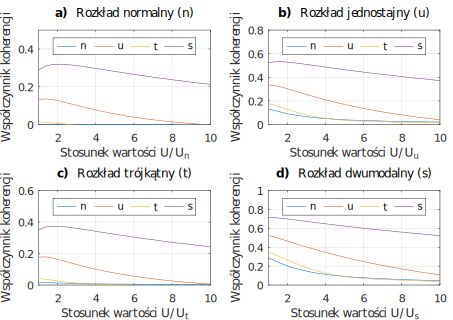
\includegraphics{obrazki/shapes}
\makecaption{fig:unc_shapefac}{Zależność wartości współczynnika koherencji w funkcji stosunku wartości niepewności rozszerzonej dla pary nieskorelowanych sygnałów błędów}
\end{center}
\end{figure}

Drugim analizowanym aspektem jest założenie wynikające z centralnego twierdzenia granicznego, wobec którego wraz ze wzrostem liczby sumowanych sygnałów kształt rozkładu sygnału wypadkowego dążyć będzie do kształtu rozkładu normalnego, jeśli sygnały te nie są skorelowane i nie występuje w nich żaden sygnał dominujący. Korektę wynikającą z opisywanych założeń zaproponowano w pracy~\cite{jakubiec_system} jako:
\begin{equation}
k_{i,j} = k_{j,i} = \frac{U_{i}^{2} + U_{j}^{2}}{\sum _{k = 0} ^{N-1} U_{k}^{2}} \label{eq:unc_cohercorrb}.
\end{equation}
Korekta ta zakłada, że współczynnik koherencji powinien być tym bardziej zbliżony do zera, im więcej istnieje źródeł błędów oraz im bardziej podobne są ich parametry. Należy zauważyć, że wraz ze wzrostem liczby sygnałów błędów cechujących się podobną wartością niepewności rozszerzonej wartość wyrażenia~\eqref{eq:unc_cohercorrb} dążyć będzie do zera tym szybciej, im bardziej zbliżone są wartości niepewności analizowanych sygnałów.

Biorąc pod uwagę współczynnik kształtu dla pary rozkładów o identycznych wartościach niepewności rozszerzonej, opisany równaniem~\eqref{eq:unc_shapertwo}, korektę wynikającą z dysproporcji pomiędzy wartościami niepewności rozszerzonych sumowanych sygnałów opisaną równaniem~\eqref{eq:unc_cohercorra} oraz korektę wynikającą z założeń centralnego twierdzenia daną zależnością~\eqref{eq:unc_cohercorrb}, otrzymuje się zależność umożliwiającą oszacowanie wartości współczynników koherencji dla $N$ nieskorelowanych sygnałów błędów w postaci:
\begin{equation}
h_{i,j} = h_{j,i} = s_{i,j} \cdot p_{i,j} \cdot k_{i,j} = s_{i,j} \sqrt{\frac{\min \emb{U_{i}, U_{j}}}{\max \emb{U_{i}, U_{j}}}} \left( \frac{U_{i}^{2} + U_{j}^{2}}{\sum _{k = 0} ^{N-1} U_{k}^{2}} \right) \label{eq:unc_coher}.
\end{equation}
Na podstawie przedstawionego równania istnieje możliwość budowy macierzy koherencji, wykorzystywanej do wyznaczenia wypadkowej wartości niepewności rozszerzonej dla analizowanych sygnałów błędów zgodnie z zależnością~\eqref{eq:unc_matrix}.

Należy zauważyć, że z uwagi na możliwość wyznaczenia wartości współczynników kształtu $s_{i,j}$ niezależnie od parametrów niepewności sygnałów błędów występujących w analizowanym torze pomiarowym, zaproponowana metoda jest możliwa do stosowania w czasie działania systemu również w przypadkach, gdy parametry sygnałów ulegają zmianie. Wadą przedstawionego rozwiązania jest konieczność wstępnego wyznaczenia wartości współczynników kształtu dla wszystkich rodzajów rozkładów sygnałów błędów występujących w analizowanym torze pomiarowym. Dodatkowo, ze względu na uproszczoną formę równania~\eqref{eq:unc_cohercorra}, która nie oddaje w pełni charakteru zależności przedstawionych na rysunku~\ref{fig:unc_shapefac}, wartości oszacowanych współczynników koherencji mogą być obarczone błędem, co w efekcie będzie miało wpływ na pojawienie się błędu oszacowania wartości wypadkowej niepewności rozszerzonej.

Ostatnim wymagającym komentarza przypadkiem jest przypadek, w którym istnieją korelacje pomiędzy analizowanymi sygnałami. Zgodnie z właściwościami macierzy koherencji elementy tej macierzy, podobnie jak elementy macierzy korelacji stosowanej w równaniu~\eqref{eq:var_matrix}, przyjmować mogą wartości z zakresu $<-1;1>$. Dla pełnej dodatniej korelacji wartość współczynnika koherencji wynosić będzie $1$, natomiast dla pełnej ujemnej korelacji wartość ta wyniesie $-1$~\cite{jakubiec_redmono}. W pozostałych przypadkach, zgodnie z informacjami przytoczonymi w poprzedniej części podrozdziału, wartość współczynnika koherencji wynikać będzie z wypadkowych parametrów kształtu splatanych rozkładów oraz współczynnika korelacji. Wobec powyższych nie jest możliwe oszacowanie wartości tego współczynnika stosując metody podobne do zaproponowanych w równaniach od~\eqref{eq:unc_shapertwo} do~\eqref{eq:unc_cohercorrb}. W omawianych sytuacjach, do wyznaczania wartości współczynników koherencji, zastosować należy metodę opisaną w pracy~\cite{jakubiec_reductive}. Inną drogą może być również przeprowadzenie analizy z osobna dla grup skorelowanych sygnałów, a następnie wykorzystanie wyznaczonych parametrów w równaniu~\eqref{eq:unc_matrix}.

Aby zweryfikować zasadność przedstawionych zależności oraz możliwość aplikacji zaproponowanej metody, przeprowadzono eksperyment metodą Monte-Carlo, którego celem było porównanie wartości niepewności rozszerzonej $U_{s}$ uzyskiwanej na drodze eksperymentu, zgodnie z instrukcją~\cite{jcgm_montecarlo}, oraz wartości $U_{c}$ uzyskiwanych zgodnie z równaniem~\eqref{eq:unc_matrix} dla współczynników koherencji wyznaczanych na podstawie równania~\eqref{eq:unc_coher}. Błąd względny $\delta_{U}$ oszacowania wartości niepewności rozszerzonej, wyrażony w procentach, będzie zatem definiowany w postaci:
\begin{equation}
\delta_{U} =  \frac{U_{c} - U_{s}}{U_{s}} \cdot 100\% \label{eq:unc_error}.
\end{equation}
W ramach eksperymentu generowano $N$ niezależnych sygnałów, których realizacje pobierane były z populacji o rozkładach $c_{i}$ i parametrach niepewności rozszerzonej $U_{i}$, których kolejne realizacje sumowano:
\begin{equation}
e_{\Sigma} \emb{k} = \sum _{i=0} ^{N-1} e_{i} \emb{k} \label{eq:unc_testsignal}.
\end{equation}
Dla uzyskanego sygnału, składającego się ze stu tysięcy próbek, wyznaczano niepewność rozszerzoną $U_{s}$ zgodnie z równaniem~\eqref{eq:unc_summation} oraz wartość $U_{c}$ oszacowaną na podstawie równania~\eqref{eq:unc_matrix} w celu wyznaczenia zgodnie z równaniem~\eqref{eq:unc_error} względnego błędu oszacowania wartości analizowanej wielkości. Opisywany proces powtarzano sto tysięcy razy, przy czym wartość $N$ pobierana była dla każdej iteracji z populacji danej przedziałem $<3,9>$ o jednakowym prawdopodobieństwie uzyskania każdej z wartości. Populacje kolejnych sygnałów $e_{i}$ stanowiły losowo kombinację rozkładów: normalnego, jednostajnego, trójkątnego i dwumodalnego, natomiast wartości niepewności rozszerzonej $U_{i}$ losowane były z przedziału $<U_{min};U_{max}>$ o jednakowym prawdopodobieństwie uzyskania każdej z wartości. Aby zweryfikować, w jakim stopniu zaproponowany w równaniu~\eqref{eq:unc_cohercorra} współczynnik korekty wpłynął na skuteczność opisanej w równaniu~\eqref{eq:unc_matrix} metody, eksperyment przeprowadzono dwukrotnie: stosując wartości współczynników koherencji wyznaczanych zgodnie z równaniem~\eqref{eq:unc_cohercorra} oraz po raz drugi, przyjmując wartość $p_{i,j} = 1$ dla dowolnej kombinacji $i$ oraz $j$. Na podstawie uzyskiwanych realizacji błędu opisanego równaniem~\eqref{eq:unc_error} sporządzano histogramm na którego podstawie oszacowano niepewność rozszerzoną analizowanej wielkości.

Ze względu na dużą zmienność parametrów sumowanych sygnałów zaproponowany eksperyment powinien w sposób miarodajny określić typową rozbieżność pomiędzy rzeczywistą, a oszacowaną za pomocą omawianej metody wartością niepewności rozszerzonej. Rysunek~\ref{fig:hist_reductive} przedstawia uzyskane histogramy względnego błędu oszacowania wypadkowej wartości niepewności rozszerzonej, natomiast w tabeli~\ref{tab:comp_reductive} przedstawiono porównanie uzyskanych wartości niepewności rozszerzonej błędu oszacowania wartości wypadkowej niepewności rozszerzonej w zależności od stosowania korekty zaproponowanej w równaniu~\eqref{eq:unc_cohercorra}, wyznaczone zgodnie z~\cite{jcgm_guide, jcgm_montecarlo}. Analizując wyniki przeprowadzonego eksperymentu zauważyć można, że wprowadzenie proponowanej korekty powoduje zmniejszenie szacowanej wartości niepewności rozszerzonej, a także zmniejszenie rozrzutu względnego błędu oszacowania tej wielkości. W efekcie możliwe jest oszacowanie wartości wypadkowej niepewności rozszerzonej z błędem względnym mieszczącym się w przedziale $\pm 5\%$.

\begin{table}[htb!]
\begin{center}
\makecaption{tab:comp_reductive}{Zestawienie wartości niepewności względnego błędu szacowania wypadkowej wartości niepewności rozszerzonej w zależności od stosowania zaproponowanej w pracy korekty współczynnika kształtu}
\begin{tabular}[c]{| c | S[table-format = +1.2] | S[table-format = +1.2] | S[table-format = +1.2] | S[table-format = +1.2] | S[table-format = +1.2] | S[table-format = +1.2] | S[table-format = +1.2] | S[table-format = +1.2] |} \hline
\textbf{$U_{i}$} & \multicolumn{2}{c|}{\textbf{a) $<1;3>$}} & \multicolumn{2}{c|}{\textbf{b) $<1;6>$}} & \multicolumn{2}{c|}{\textbf{c) $<1;10>$}} & \multicolumn{2}{c|}{\textbf{d) $<1;20>$}} \\ \hline
\textbf{$\delta_{U}$} & \textbf{$U_{-}$} & \textbf{$U_{+}$} & \textbf{$U_{-}$} & \textbf{$U_{+}$} & \textbf{$U_{-}$} & \textbf{$U_{+}$} & \textbf{$U_{-}$} & \textbf{$U_{+}$} \\ \hline
Z korektą   & -2.23 & +4.83 & -2.43 & +4.59 & -2.54 & +4.52 & -2.62 & +4.45 \\ \hline
Bez korekty & -1.14 & +7.96 & -1.13 & +8.69 & -1.09 & +8.80 & -1.13 & +8.86 \\ \hline
\end{tabular}
\end{center}
\end{table}

\begin{figure}[htb!]
\begin{center}
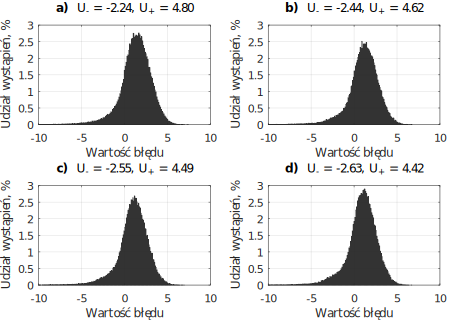
\includegraphics{obrazki/hist_reductive}
\makecaption{fig:hist_reductive}{Histogramy względnego błędu oszacowania wypadkowej wartości niepewności rozszerzonej dla zaproponowanej w pracy metody odpowiadające danym zestawionym w tabeli~\ref{tab:comp_reductive}}
\end{center}
\end{figure}

Analizując przedstawione dotychczas zależności zauważyć można, że sposób opisu niedokładności wyniku pomiaru zależeć będzie w dużej mierze od potrzeb projektanta toru pomiarowego oraz od specyfiki zakłócających proces pomiaru zjawisk. Opis wykorzystujący wariancję sygnału błędu wydaje się bardziej przystępny i mniej skomplikowany, a dodatkowo wielkość ta może być utożsamiana z mocą sygnału~\cite{proakis_dsp}. Opis wykorzystujący niepewność rozszerzoną będzie jednak bardziej precyzyjny, ze względu na informacje odnośnie prawdopodobieństwa wystąpienia danej wartości realizacji sygnału błędu, natomiast wymaga on większego zaangażowania w proces wyznaczania ostatecznej wartości tej wielkości. W odpowiednich okolicznościach, jeżeli spełnione są warunki związane z centralnym twierdzeniem granicznym, opis bazujący na wariancji sygnału błędu może być w łatwy sposób przeniesiony na opis związany z niepewnością rozszerzoną~\cite{jcgm_guide}.

Wyznaczone zgodnie z metodą redukcyjnej arytmetyki interwałowej szacowane wartości niepewności rozszerzonej mogą w niewielkim stopniu odbiegać od wartości rzeczywistych, co opisano w~\cite{jakubiec_arithmetic, jakubiec_model}. Zaproponowana w równaniu~\eqref{eq:unc_cohercorra} korekta zmniejsza omawiane różnice, zapewniając jednocześnie niski stopnień skomplikowania obliczeń oraz względny błąd oszacowania wypadkowej wartości niepewności rozszerzonej nieprzekraczający $\pm 5\%$ prawidłowej wartości tej wielkości. Można zatem stwierdzić, że zaproponowana w pracy metoda szacowania wypadkowej wartości niepewności rozszerzonej jest zasadna z punktu widzenia przyjętych założeń. Ponadto, ze względu na niską złożoność obliczeń, metoda ta może być stosowana w przypadkach, gdzie liczba analizowanych sygnałów oraz ich parametry ulegają zmianie.

\section{Algorytm jako fragment toru pomiarowego}

Podczas opisu właściwości cyfrowej części toru pomiarowego przedstawiono przypadek, w którym analizowany obiekt przetwarzał kolejne próbki sygnału wejściowego na próbki sygnału wyjściowego zgodnie z odpowiadającą mu transmitancją i funkcją przetwarzania. Algorytmy stosowane w torach pomiarowych mogą generować wiele wielkości wyjściowych, pobierając przy tym w oknie pomiarowym określoną liczbę próbek wielkości wejściowych. W przypadku, gdy wyjście analizowanego obiektu stanowi $M$ próbek wielkości wyjściowych wyznaczanych na podstawie $N$ próbek wielkości wejściowych, a funkcja przetwarzania tego obiektu jest liniowa, działanie obiektu przedstawić można w ogólnej postaci jako~\cite{jakubiec_algorithms, jakubiec_single}:
\begin{equation}
\begin{bmatrix}
X \emb{0}   \\
X \emb{1}   \\
\vdots      \\
X \emb{M-1}
\end{bmatrix}
=
\begin{bmatrix}
a_{0, 0}   &   a_{0, 1} &   \cdots   &   a_{0, N-1}      \\
a_{1, 0}   &   \ddots   &            &   a_{1, N-1}      \\
\vdots     &            &   \ddots   &   \vdots          \\
a_{M-1, 0} &   \cdots   &   \cdots   &   a_{M-1, N-1}
\end{bmatrix}
\begin{bmatrix}
x \emb{0}   \\
x \emb{1}   \\
\vdots      \\
x \emb{N-1}
\end{bmatrix}
\label{eq:alg_out_mat},
\end{equation}
gdzie $a_{i,j}$ to kolejne współczynniki macierzy transformacji. Równanie~\eqref{eq:alg_out_mat} można przedstawić również w postaci iloczynu~\cite{jakubiec_algorithms}:
\begin{equation}
\mathbf{X} = \mathbf{A} \cdot \mathbf{x} \label{eq:alg_out_mul},
\end{equation}
gdzie $\mathbf{X}$ jest wektorem wielkości wyjściowych, $\mathbf{A}$ macierzą transformacji oraz $\mathbf{x}$ wektorem wielkości wejściowych. Wobec powyższych zależności, pojedynczą wielkość wyjściową algorytmu przedstawić można w postaci:
\begin{equation}
X \emb{i} = a_{i, 0} x \emb{0} + a_{i, 1} x \emb{1} + \hdots + a_{i, N-1} x \emb{N-1} \label{eq:alg_out_single}.
\end{equation}
Na podstawie równania~\eqref{eq:alg_out_single} zauważyć można, że analizowany obiekt stanowi zbiór filtrów o skończonej odpowiedzi impulsowej \enquote{FIR}. Przedstawione metody analizy będą zatem przypominały metody analizy opisywanego typu filtru~\cite{mehrnia_fir}.

Wartości współczynników macierzy transformacji opisanej równaniem~\eqref{eq:alg_out_mat} mogą nie być znane przez projektanta toru pomiarowego, jeżeli w torze pomiarowym stosowany jest algorytm o nieznanej strukturze numerycznej. Ich znajomość jest jednak konieczna w celu przeprowadzenia analizy metrologicznej zastosowanego algorytmu. Najczęściej projektant toru pomiarowego stosuje gotowy algorytm, zaimplementowany np. w środowisku \enquote{GNU Octave}, \enquote{Matlab} lub dostarczany mu jako zewnętrzną bibliotekę języka programowania~\cite{pruuvsa_dwt}. W takim przypadku należy przeprowadzić proces identyfikacji wartości współczynników macierzy, który przedstawiono w dalszej części rozdziału. Drugim przypadkiem jest sytuacja, w której wartości współczynników mogą być wyznaczone analitycznie za pomocą odpowiednich zależności, opisujących stosowany algorytm. Możliwy jest również przypadek, w którym znana jest transmitancja $H_{i}(z)$ dla kolejnych wielkości wyjściowych, przy czym wyznaczenie wartości współczynników macierzy transformacji odbywać się będzie poprzez przekształcenie tej transmitancji na postać zgodną z równaniem~\eqref{eq:alg_out_single}.

Identyfikacja wartości współczynników macierzy transformacji w przypadku istniejącego algorytmu polega na wyznaczaniu odpowiedzi tego algorytmu dla wektora wielkości wejściowych o wartościach zgodnych z równaniem~\cite{jakubiec_algorithms, jakubiec_system}:
\begin{equation}
x \emb{n} =
\begin{cases}
	1 & $gdy$~n = i \\
	0 & $gdy$~n \neq i
\end{cases}
\label{eq:wt_ident},
\end{equation}
przy czym uzyskany wektor wielkości wyjściowych stanowi $i$-tą kolumnę macierzy transformacji tego algorytmu. Przedstawioną operację należy wykonać dla wszystkich kolumn macierzy transformacji, a zatem dla $i$ w przedziale $<0;N-1>$. Opisana metoda jest uniwersalna, przy czym wymaga ona, aby identyfikowany algorytm spełniał założenia przedstawione na początku podrozdziału.

Aby ustalić związek pomiędzy sygnałami błędów wielkości wejściowych, a sygnałami błędów wielkości wyjściowych analizowanego algorytmu, należy przeanalizować proces wyznaczania wartości pojedynczej wielkości wyjściowej. Zakładając, że wielkości wejściowe algorytmu są obarczone błędami o charakterze addytywnym zgodnie z zależnością:
\begin{equation}
\tilde{x} \emb{i} = \dot{x} \emb{i} + e_{x,\Sigma} \emb{i} = \dot{x} \emb{i} + e_{x,s} \emb{i} + e_{x,d} \emb{i} + e_{x,r} \emb{i} \label{eq:alg_inputval},
\end{equation}
gdzie $e_{x,s}(i)$ oznacza błąd statyczny, $e_{x,d}(i)$ błąd dynamiczny oraz $e_{x,r}(i)$ błąd losowy wielkości wejściowej, istnieje możliwość osobnej analizy wyniku realizacji algorytmu dla idealnych wartości wielkości wejściowych oraz dla wymienionych sygnałów błędów. Błąd wielkości wyjściowej przenoszony z wejścia na wyjście algorytmu można zatem opisać, zgodnie z równaniem~\eqref{eq:alg_out_single}, w postaci:
\begin{equation}
e_{X,p} \emb{i} = a_{i, 0} e_{x,\Sigma} \emb{0} + a_{i, 1} e_{x,\Sigma} \emb{1} + \hdots + a_{i, N-1} e_{x,\Sigma} \emb{N-1} \label{eq:alg_outerr}.
\end{equation}

Dla sygnałów błędów o charakterze statycznym, ze względu na fakt że wartość realizacji tych sygnałów jest niezmienna w obrębie pojedynczego okna pomiarowego, równanie~\eqref{eq:alg_outerr} można uprościć i zapisać w postaci:
\begin{equation}
e_{X,s} \emb{i} = a_{i, 0} e_{x,s} \emb{k} + a_{i, 1} e_{x,s} \emb{k} + \hdots + a_{i, N-1} e_{x,s} \emb{k} = e_{x,s} \emb{k} \sum _{j = 0} ^{N-1} a_{i, j} \label{eq:alg_outerr_stat},
\end{equation}
gdzie $e_{x,s}(k)$ jest błędem statycznym wielkości wejściowej dla $k$-tego numeru okna, natomiast $e_{X,s}(i)$ błędem statycznym wielkości wyjściowej algorytmu. Powtarzając proces wyznaczania wartości wielkości wyjściowej algorytmu wielokrotnie, dla różnych numerów okna pomiarowego realizacje sygnału błędu statycznego mogą przyjmować różne wartości. W takim przypadku wyjściowy błąd statyczny również można rozpatrywać w kategoriach probabilistycznych, a jego wariancję opisać można równaniem uwzględniającym wariancję sygnału wejściowego błędu statycznego:
\begin{equation}
\sigma_{X,s}^{2} \emb{i} = \sigma_{x,s}^{2} \left( a_{i, 0} + a_{i, 1} + \hdots + a_{i, N-1} \right)^{2} = \sigma_{x,s}^{2} \left( \sum _{j = 0} ^{N-1} a_{i, j} \right)^{2} \label{eq:alg_outvar_stat}.
\end{equation}
Należy zauważyć, że kształt rozkładu wyjściowego błędu statycznego będzie identyczny, jak kształt rozkładu błędu statycznego na wejściu algorytmu.

Dla sygnałów błędów dynamicznych należy przeprowadzić analizę zgodnie z metodologią przedstawioną w poprzedniej części rozdziału, wykorzystując znajomość transmitancji $H_{i}(z)$ odpowiedniej dla analizowanej wielkości wyjściowej algorytmu. Identycznie, jak w przypadku równania~\eqref{eq:mid_disc_err_dyn_prop}, wyznaczyć należy wypadkowe amplitudy oraz przesunięcia w fazie kolejnych harmonicznych sygnału propagowanego błędu dynamicznego, a następnie wykorzystać należy równania od~\eqref{eq:dyn_harm} do~\eqref{eq:dyn_corr} w celu wyznaczenia wariancji analizowanych sygnałów. Transmitancja $H_{i}(z)$ dla $i$-tej wielkości wyjściowej może zostać wyznaczona na podstawie wartości współczynników $i$-tego wiersza macierzy transformacji algorytmu jako:
\begin{equation}
H_{i} \emb{z} = a_{i, 0} + a_{i, 1} z^{-1} + \hdots + a_{i, N-1} z^{-N+1} = \sum _{k = 0} ^{N-1} a_{i, k} z^{-k} \label{eq:alg_trans_single}.
\end{equation}
W omawianym przypadku przyjmuje się, że algorytm posiada idealną transmitancję i nie wprowadza do sygnału wyjściowego błędu dynamicznego własnego.

W przypadku błędów o charakterze losowym, wykonując algorytm wielokrotnie, uzyskać można zależność wiążącą wariancję błędu na wyjściu algorytmu z wariancją błędów wielkości wejściowych. Zakładając, że wszystkie wielkości wejściowe algorytmu pochodzą z tej samej cześć toru pomiarowego, a zatem ich parametry statystyczne są identyczne, oraz że kolejne błędy wielkości wejściowych nie są ze sobą skorelowane, zależność tą opisać można jako:
\begin{equation}
\sigma_{r}^{2} \emb{i} = a_{i, 0}^{2} \sigma_{x,r}^{2} + a_{i, 1}^{2} \sigma_{x,r}^{2} + \hdots + a_{i, N-1}^{2} \sigma_{x,r}^{2} = \sigma_{x,r}^{2} \sum _{j=0} ^{N-1} {a_{i, j}^{2}} \label{eq:alg_outvar_rand}.
\end{equation}

Poza przenoszeniem przez algorytm błędów zawartych w wielkościach wejściowych na jego wyjście, algorytm wprowadza do wielkości wyjściowych błędy własne. Błędy te wynikają niedokładności wyznaczenia współczynników algorytmu oraz z przeprowadzanych podczas obliczeń zaokrągleń. Ich wartości będą zatem uzależnione od wielu czynników, a ich analiza powinna odbywać się indywidualnie dla zaimplementowanego algorytmu. Zakładając, że wyznaczanie wartości $i$-tej wielkości wyjściowej algorytmu odbywać się będzie wielokrotnie, błędy własne opisywać można w kategorii probabilistycznej za pomocą związanej z nimi wariancji $\sigma_{X,z}^{2}(i)$. Ze względu na fakt, że liczba operacji mnożenia i dodawania, odpowiedzialnych za powstawanie omawianej grupy błędów będzie duża ($N$ mnożeń oraz $N$ dodawań) błąd ten będzie miał rozkład zbliżony do normalnego~\cite{jcgm_guide}. W przypadku, gdy na etapie identyfikacji wartości macierzy współczynników uzyskano wartości obarczone błędami, należy rozszerzyć analizę o przedstawienie konsekwencji tego zjawiska. W takim przypadku należy przeanalizować wprowadzany do wielkości wyjściowych statyczny błąd własny oraz wykonać analizę dla błędów własnych dynamicznych, analogicznie jak opisano równaniem~\eqref{eq:mid_disc_err_dyn_self}. Omawiany przypadek nie będzie rozpatrywany w pracy, ponieważ identyfikując wartości macierzy transformacji za pomocą przedstawionego algorytmu lub wyznaczając ich wartości przy użyciu odpowiednich funkcjonałów, wprowadzany błąd wynikać będzie głównie z zaokrągleń i będzie można analizować go równolegle z wprowadzanym losowym błędem $e_{X,z}$. Omawianą analizę przedstawia szczegółowo praca~\cite{jakubiec_system}.

Wobec powyższych założeń, w celu wyznaczenia wariancji $\sigma_{X,\Sigma}^{2}(i)$ wypadkowego błędu $e_{X,\Sigma}(i)$ dla $i$-tej wielkości wyjściowej analizowanego algorytmu należy wykorzystać zależność~\eqref{eq:var_matrix}, przy czym przyjmuje ona w tym przypadku postać:
\begin{equation}
\sigma_{X,\Sigma}^{2} \emb{i} =
\begin{bmatrix}
\sigma_{X,s} \emb{i} \\ \sigma_{X,d} \emb{i} \\ \sigma_{X,r} \emb{i} \\ \sigma_{X,z} \emb{i}
\end{bmatrix}^{T}
\begin{bmatrix}
1         & r_{d,s} & r_{r,s} & r_{z,s} \\
r_{s,d}   & 1       & r_{r,d} & r_{z,d} \\
r_{s,r}   & r_{d,r} & 1       & r_{z,r} \\
r_{s,z}   & r_{d,z} & r_{r,z} & 1
\end{bmatrix}
\begin{bmatrix}
\sigma_{X,s} \emb{i} \\ \sigma_{X,d} \emb{i} \\ \sigma_{X,r} \emb{i} \\ \sigma_{X,z} \emb{i}
\end{bmatrix}
\label{eq:alg_outvar_mat},
\end{equation}
gdzie $r_{i,j}$ stanowi współczynnik macierzy korelacji dla wybranych błędów cząstkowych analizowanego algorytmu. Wyznaczenie niepewności rozszerzonej może być przeprowadzone zgodnie z zależnością~\eqref{eq:unc_matrix}, przekształconą do postaci:
\begin{equation}
U_{X,\Sigma} \emb{i} = \sqrt{
\begin{bmatrix}
U_{X,s} \emb{i} \\ U_{X,d} \emb{i} \\ U_{X,r} \emb{i} \\ U_{X,z} \emb{i}
\end{bmatrix}^{T}
\begin{bmatrix}
1         & h_{d,s} & h_{r,s} & h_{z,s} \\
h_{s,d}   & 1       & h_{r,d} & h_{z,d} \\
h_{s,r}   & h_{d,r} & 1       & h_{z,r} \\
h_{s,z}   & h_{d,z} & h_{r,z} & 1
\end{bmatrix}
\begin{bmatrix}
U_{X,s} \emb{i} \\ U_{X,d} \emb{i} \\ U_{X,r} \emb{i} \\ U_{X,z} \emb{i}
\end{bmatrix}}
\label{eq:alg_outunc_mat},
\end{equation}
przy czym $h_{i,j}$ oznacza współczynnik koherencji wyznaczany zgodnie z zależnością~\eqref{eq:unc_coher}. Należy zauważyć, że równania~\eqref{eq:alg_outvar_mat} oraz~\eqref{eq:alg_outunc_mat} mogą zawierać inną liczbę elementów, niż wskazano. Dokładna postać przedstawionych równań zależeć będzie od budżetu niepewności wielkości wejściowych analizowanego algorytmu.

Na podstawie równań~\eqref{eq:alg_outvar_stat} oraz~\eqref{eq:alg_outvar_rand} wprowadzić można dodatkowe wielkości przedstawione następującymi zależnościami:
\begin{gather}
A_{i,s} = \sum _{j = 0} ^{N-1} a_{i, j} \label{eq:alg_trans_stat}, \\
A_{i,r} = \sqrt{\sum _{j = 0} ^{N-1} a_{i, j}^{2}} \label{eq:alg_trans_rand},
\end{gather}
gdzie $A_{i,s}$ jest współczynnikiem przenoszenia dla błędów statycznych, natomiast jest $A_{i,r}$ współczynnikiem przenoszenia dla błędów losowych $i$-tej wielkości wyjściowej analizowanego algorytmu. Wyznaczenie wartości opisanych współczynników umożliwi wyznaczenie wariancji kolejnych błędów losowych oraz statycznych, a dodatkowo będzie stanowiło informacje, w jaki sposób analizowany algorytm przenosi z wejścia na wyjście określony rodzaj błędu. Można zauważyć, że dla niskich wartości współczynnika przenoszenia (tj. $A_{i} < 1$) kolejne błędy wielkości wejściowych będą tłumione (wariancja błędu wielkości wyjściowej będzie mniejsza, niż wariancja błędów wielkości wejściowych). Odwrotna sytuacja będzie miała miejsce w przypadku dużych wartości współczynnika (tj. $A_{i} > 1$).

W przypadku analizy błędów dynamicznych, na podstawie równania~\eqref{eq:alg_trans_single} po podstawieniu $z = e^{j\omega}$, wyznaczyć można adekwatne dla równań~\eqref{eq:mid_disc_amp} oraz~\eqref{eq:mid_disc_phi} zależności opisujące wzmocnienie $K_{X,i}(\omega_{n})$ oraz przesunięcie w fazie $\varphi_{X,i}(\omega_{n})$ przetwarzanych harmonicznych sygnału w funkcji pulsacji znormalizowanej $\omega_{n}$ dla $i$-tej wielkości wyjściowej algorytmu w postaci:
\begin{gather}
G_{X,i} \emb{\omega_{n}} = \sum _{k = 0} ^{N-1} a_{i,k} e^{-j k \omega_{n}} \label{eq:alg_trans_norm}, \\
K_{X,i} \emb{\omega_{n}} = \left| G_{X,i} \emb{\omega_{n}} \right| = \sqrt{\left( \Re \left( G_{X,i} \emb{\omega_{n}} \right) \right)^{2} + \left( \Im \left( G_{X,i} \emb{\omega_{n}} \right) \right)^{2}} \label{eq:alg_trans_amp}, \\
\varphi_{X,i} \emb{\omega_{n}} = \arctan \left( \frac{\Im \left( G_{X,i} \emb{\omega_{n}} \right)}{\Re \left( G_{X,i} \emb{\omega_{n}} \right)} \right) \label{eq:alg_trans_phi},
\end{gather}
przy czym pulsacja znormalizowana, oznaczona symbolem $\omega_{n}$, odnosi się do pulsacji próbkowania i jest określona przez następującą zależność:
\begin{equation}
\omega_{n} = 2\pi \frac{\omega}{\omega_{s}} \label{eq:puls_norm},
\end{equation}
gdzie $\omega$ jest analizowaną pulsacją, natomiast $\omega_{s}$ pulsacją próbkowania równą $\frac{2 \pi}{T_{p}}$ dla okresu próbkowania $T_{p}$. Prawidłowa wartość pulsacji znormalizowanej mieści się zatem w zakresie $<0;\pi>$, co odpowiada zakresowi od zera do pulsacji Nyquista dla przyjętego okresu próbkowania.

\section{Podsumowanie przedstawionych zależności}

W poprzednich częściach rozdziału przedstawiono modele kolejnych fragmentów toru pomiarowego, które opisywały związki pomiędzy błędami na wejściu i wyjściu analizowanego obiektu, a także wskazywały rolę tego obiektu we wprowadzaniu do sygnału wyjściowego błędów własnych. Zaproponowany model wprowadzał podział na statyczne i dynamiczne właściwości obiektu, które opisywane były transmitancją i funkcją przetwarzania obiektu. Opisane zaproponowanym modelem fragmenty toru pomiarowego, które zostały ze sobą połączone kaskadowo oraz cechują się addytywną funkcją przetwarzania, opisać można modelem wypadkowym oraz z osobna analizować zawarte w nim błędy cząstkowe. Zaproponowana metoda wyznaczania niepewności wypadkowej bazuje na określeniu związków pomiędzy kolejnymi niepewnościami składowymi, a następnie wykorzystuje redukcyjną arytmetykę interwałową do wyznaczenia niepewności wypadkowej. Zaproponowany opis uwzględnia ewentualne korelacje pomiędzy kolejnymi grupami błędów, a w przypadku braku tych korelacji wymaga jedynie określenia związków pomiędzy kształtem rozkładu kolejnych składanych błędów~\cite{jakubiec_reductive, batko_uncertainty}.

Przedstawiony model oceny dokładności wyniku pomiaru zakłada, że obecne w sygnale pomiarowym błędy cechują się symetrycznymi rozkładami o zerowej wartości oczekiwanej. W przypadku, gdy wartość oczekiwana realizacji błędu jest niezerowa, błąd ten posiada składową systematyczną, którą należy skorygować w ostatecznym wyniku pomiaru. Jeżeli nie jest spełnione założenie odnośnie symetrii rozkładów składanych błędów, to do określenia rozkładu błędu wynikowego należy stosować metodę analityczną bazującą na wyznaczeniu splotu składanych funkcji gęstości prawdopodobieństwa lub wykorzystać metodę Monte-Carlo, która jest zwykle bardziej przystępna i optymalna ze względu na mniejszy stopień skomplikowania~\cite{janssen_montecarlo, roj_annuncertainty}.

Przeprowadzone rozważania nie poruszały problemu opóźnień w systemach pomiarowo-sterujących, a zatem nie brano w nich pod uwagę błędów związanych z opóźnieniami. Tematyka ta nie będzie poruszana w dalszych częściach pracy. Warto jednak zauważyć, że zaproponowany model błędu może być z łatwością dopasowany do możliwości analizy właściwości i wpływu tych błędów na niedokładność wielkości wyjściowych. Należy wtedy uwzględnić w modelu dodatkowy składnik błędu, który definiować można zgodnie z metodą zaproponowaną w~\cite{wymyslo_delay, jakubiec_system}. Z punktu widzenia zaproponowanego modelu, zjawisko to opisać można jako dodatkowe przesunięcie w fazie składowych przetwarzanego sygnału, będące iloczynem pulsacji analizowanej harmonicznej i wartości realizacji błędu opóźnienia.
